\documentclass[11pt]{article} % font size
\usepackage{fancyhdr}
\usepackage{extramarks}
\usepackage{dcolumn}
\usepackage{amsthm}
\usepackage{authblk}
\usepackage{amsfonts}
\usepackage{color}
\usepackage[dvipsnames]{xcolor}
\usepackage{tikz}
\usetikzlibrary{arrows,positioning,decorations.pathreplacing}
%\usetikzlibrary{decorations.pathreplacing}
\usepackage[utf8]{inputenc}
\usepackage[margin=1.0in]{geometry} % side-page margin 
\usepackage{amsmath, latexsym}
\usepackage{changepage}
\usepackage{amssymb}
\usepackage{enumitem}
\usepackage{float}
\usepackage{comment}
\usepackage{booktabs}
\renewcommand{\baselinestretch}{1.2} % line spacing 
\usepackage{subcaption}
\usepackage{graphicx}
\usepackage{xifthen}
\usepackage{calc}
\usepackage{breqn}
\usepackage{mathtools}
\usepackage{longtable}
\usepackage{caption}
\usepackage{xcolor} % text color
% \graphicspath{ {figures/} }
% \usepackage{array}
\def\changemargin#1#2{\list{}{\rightmargin#2\leftmargin#1}\item[]}
\let\endchangemargin=\endlist

\DeclarePairedDelimiter\ceil{\lcseil}{\rceil}
\DeclarePairedDelimiter\floor{\lfloor}{\rfloor}
\newcommand{\minus}{\scalebox{0.5}[1.0]{$-$}}

\pagestyle{fancy}
\fancyhf{}
\fancyhead[LE,RO]{\textit{\small{Commercial Mortgage Distress During the COVID-19 Pandemic}}}
\fancyhead[RE,LO]{\footnotesize{\leftmark}}
\fancyfoot[CE,LO]{}
\fancyfoot[LE,RO]{\thepage}

\renewcommand{\headrulewidth}{0.5pt}
\renewcommand{\footrulewidth}{0.0pt}



\usepackage{hyperref}
\hypersetup{
    colorlinks=true,
    linkcolor=black,
    filecolor=Mulberry,      
    urlcolor=blue,
}
\urlstyle{same}

%%%%%%%%%%%%%%%%%%%%%%%%%%%%%%%%%%%%%%%%%%%
\begin{document}
\thispagestyle{empty}
\title{\vspace{-0.0em}Commercial Mortgage Distress during the COVID-19 Pandemic: \\ Evaluating the Impact of Government Aid and Mobility}
\author{\vspace{2em} By: \\ \vspace{-0.5em} \textbf{William Carpenter}}
\date{\vspace{25em} \normalsize{Submitted to Princeton University} \\ Department of Economics \\ In Partial Fulfillment of the Requirements for the A.B. Degree \\ \vspace {3.0em} April 14\textsuperscript{th}, 2021}
\maketitle
\thispagestyle{empty}
% ADD ABSTRACK BACK HERE
%\vspace{-1.0em}
\newpage
\textcolor{white}{fill}\vspace{5em}
\begin{abstract}
\small
This paper investigates how government aid and mobility affected the likelihood of financial distress for commercial mortgages during the COVID-19 pandemic by utilizing asset-backed security data on loan performance from 2019--2021. Commercial real estate is an industry that has experienced a substantial and prolonged disruption from the pandemic's economic consequences within the United States. For government aid, a dual perspective is employed by considering county-level measures of uptake activity for the Paycheck Protection Program (PPP) and Economic Injury Disaster loans (EIDL).  Mobility is measured at the county-level using government data on daily transportation. Analysis of how these factors impacted loan distress during the pandemic is also  broken down by property type to evaluate heterogeneity across different industries. Main findings for PPP uptake activity suggest that higher amounts of funding and loans appear to flow to counties with more negatively affected commercial properties, particularly in the case of retail and lodging, but they do not play a significant role overall in reducing probability of loan distress. These results supplement a growing body of literature  that has primarily focused on the ability of the PPP to bolster employment. In contrast, when considering distress measures based on loan delinquencies, EIDL activity is found to correspond with lower overall loan distress during the pandemic. This provides some evidence about the efficacy of a program that has received less research attention than the PPP and is aimed at supporting operating expenses, rather than specifically targeting payroll. Finally, results for within-county shifts in population mobility during the pandemic period indicate that the financial well-being of commercial mortgages is adversely impacted by declines in travel. Effects of mobility were most robust for retail, office, and lodging properties. These findings are perhaps most applicable to policymakers and researchers seeking to assess the transmission of government policies during the pandemic. They are also potentially useful for those concerned with ongoing credit risk factors in the commercial real estate market.
\\ \\ \\
\normalsize
\noindent
\textbf{Keywords:} commercial mortgages, COVID-19, distress, PPP, EIDL, mobility \\
\end{abstract}

\vspace{0.5em}
\thispagestyle{empty}

% \normalsize
% \newpage
% \section*{Acknowledgements}
% \thispagestyle{empty}
% First and foremost, I would like to express my deep and sincere gratitude to my parents for all their support. The opportunity to embark on this research project has been informative and enlightening, for which I am very grateful to the Economics Department at Princeton for making possible. Guidance from my advisor, Professor Adrien Matray, has been invaluable and I thank him for his constant engagement over these past nine months. I am very glad to have met my close friends and classmates in part through this research process, Tiger Gao and Ricarrdo Lapi, who have both have been an inspiration to me while studying economics.

% I would also like to acknowledge Firestone Library and the Data and Statistical Services Lab (DSS) for being wonderful resources for my research as an undergraduate. Both are foundational for the success of empirical economics research at Princeton. Oscar Torres Reyna has exceptional prowess with statistical software, deftly handling my questions and concerns more times than I can remember. I commend the resiliency of the entire DSS staff during the pandemic, where they successfully overcame many logistical difficulties and made help readily accessible over the course of a very unique year. And when I found myself in a hectic search for data, no issue was too complex for Bobray Bordelon or Barbara Coffey at Firestone, both of whom deserve all the credit they receive and more for assisting so many students. 

% Finally, much of this research would simply not have been possible without access to a few key pieces of software. Many, many thanks to Finsight for their publicly accessible data platform. It has certainly helped to illuminate today's capital markets and is one of the main reasons why I have been able to explore the world of securitization so profusely over this past year. I sincerely hope the data will underpin more research on asset-backed securities and the pandemic in the near future. I am thankful to Stata Corp. for excellent statistical software that I used every step of the way to organize and analyze data. My final thanks is to Overleaf for providing a phenomenal \LaTeX  \hspace{0.2em}editor. It will certainly continue to be an indispensable tool of many economists for years to come. 

\newpage
\thispagestyle{empty}
\tableofcontents
\vspace{3.5em}
\listoftables
\thispagestyle{empty}
\newpage

% \hypersetup{
%     colorlinks=true,
%     linkcolor=black, % MidnightBlue
%     filecolor=magenta,      % Magenta 
%     urlcolor=black,        % Purple
%     citecolor=black, % MidnightBlue
% }

\hypersetup{
    colorlinks=true,
    linkcolor=MidnightBlue, % MidnightBlue
    filecolor=magenta,      % Magenta 
    urlcolor=Purple,        % Purple
    citecolor=MidnightBlue, % MidnightBlue
}

\noindent 
\normalsize

\section{Introduction}
% RWYA. granular, pervasive, microcosm, efficacy, encompass, stringent, comprehensive, capitulation, in the circumstance, instances of...,  encompass, indicator variable. `Financial hardship' or `distress.'  New channels should be studied beyond usual factors, like mobility and business-type exposure. 

The COVID-19 pandemic has had a momentous effect on economic stability within the United States and worldwide. The speed and severity of the health crisis produced widespread economic uncertainty that quickly roiled markets, prompting record high unemployment rates and asset price volatility. Declaration of a national emergency in the U.S. deterred consumer activity and became the catalyst for many local governments to enact unprecedented restrictions on social interactions, causing widespread business disruption. The announcement was also quickly followed by a robust wave of fiscal and monetary stimulus intended to address the adverse effects of the virus on individuals and businesses countrywide. 

Commercial real estate (CRE) is one industry that has been severely disrupted by these drastic changes, particularly the financial stability of commercial mortgages that underpin many large businesses countrywide. Since March 2020, economic downturn in the U.S. has prompted a marked increase in loan delinquency rates, signaling that borrowers are struggling to make their scheduled monthly payments. These rates quickly reached near all-time highs in the mid-summer of 2020 (\hyperlink{Trepp}{Trepp} 2021).\footnote{\href{https://www.trepp.com/}{Trepp} research data indicates that CMBS 30+ day delinquency rates spiked to a peak of 10.3\% from about 2.0\% before the pandemic began. This peak was slightly lower than what was reached during a CRE market meltdown during 2012, in wake of the 2008 financial crisis.} Lodging, retail, and mixed-use enterprises in particular have had difficulties from non-essential business restrictions and a rapid decline in travel. Office space has been adversely affected by new safety precautions and technological capabilities that have favored remote work options. Other common property types, like industrial production plants and warehouses, have been relatively more insulated from negative effects in part from a lack of direct consumer interaction and high demand for home delivery services.  

A research lens focused on the CRE turmoil caused by the pandemic is imperative. After one year since the virus reached the U.S., indications of a broad market recovery remain alarmingly sparse. Delinquency rates are still elevated and far above pre-pandemic levels.\footnote{\hyperlink{Trepp}{Trepp} (2021) most recent data for its aggregate CMBS index show that delinquency levels are about 6.6\% for February 2021.}  This situation is concerning for many possible reasons. New virus variants and outbreaks still threaten to intensify social and business restrictions across the country in early 2021. Persisting low demand for travel and brick-and-mortar commerce could continue to excessively strain many businesses, even those that have managed to support themselves well through the first year of the pandemic. In contrast to residential real estate markets, CRE also has not seen the same degree of direct assistance from the Federal Government for forbearance and payment deferral. Other assistance offered by the Federal Reserve has been problematic in terms of eligibility for commercial property owners (\hyperlink{Fedor}{Fedor \& Rennison} 2020, \hyperlink{Scott}{Scott} 2020[1]). Deterioration of debt within the CRE market could ultimately pose a major systemic risk for U.S. financial markets. For example, \hyperlink{Scott}{Scott} (2020[1]) noted that current exposure is high with about 39\%, or \$1 trillion, of CRE loans being held within bank portfolios.\footnote{Statistics are sourced from 2019 data. Another 15\% of the total CRE loan market is also held by life insurance companies. \hyperlink{Scott}{Scott} 2020[1] point out that interconnectedness in real estate financing can have drastic consequences, a risk that already manifested itself during the Great Recession in 2008 with residential mortgages and subprime financing practices.} Increased stress from the pandemic could also expose issues with poor underwriting standards in the commercial mortgage market (\hyperlink{Griffin}{Griffin \& Priest} 2020). Finally, from a long-term perspective, a more permanent shift away from physical space could proliferate vacancies and erode property market values, potentially causing many loans to go underwater in the future. The effect of government aid and a broader economic recovery could be crucial in mitigating these risks.

This paper seeks to contribute to literature on COVID-19 by investigating how government aid and mobility impacted distress within commercial mortgages, an innate aspect of the CRE market. Publicly available performance data for conduit loans is obtained for a variety of common property types and provides a suitable time period of analysis from Jan. 2019 - Feb. 2021. From the data, three different definitions for loan distress are constructed that address some variations in financial severity.\footnote{These measures are discussed in further detail within the methodology section.} For government aid, the two programs of focus are the Paycheck Protection Program (PPP) and Economic Injury Disaster Loans (EIDL). Both were implemented by the Small Business Administration (SBA) to support business financial stability in response to the pandemic, with PPP dedicated mainly to payroll needs and EIDL to operating expenses. Each program was available for eligible businesses across the country and could have been utilized, indirectly or directly, by many tenants and CRE borrowers to make scheduled rent payments.\footnote{The PPP was designed to support payroll but funds could be used for other purposes. \hyperlink{Granja}{Granja et al.} (2020) note that many firms in their same used the funds to make fixed payments and/or to build up savings buffers.} Evaluating PPP and EIDL in tandem is also a methodology this paper intends to contribute to prevailing research, where most focus has been predominantly concentrated on the PPP. Micro-data is available for both programs and is used to create county-level measures of funding and loan coverage for businesses, which is intended to capture both the magnitude and spread of loan uptake. Mobility is derived from counts of trips that are $\geq$25 miles in order to capture trends in travel that are not highly localized and routine. Shifts in mobility could thus be a reasonable proxy for economic recovery in terms of capturing travel that could be work-based or leisured-based, potentially representing individuals going cross-county or even further.\footnote{It will be discussed in further detail in \hyperlink{Data}{Section 4} that mobility captures various forms of travel, such as: by-foot, automobile, subway, train, and aviation. This could be travel from suppliers too, not just consumers.} To address considerable heterogeneity in distress levels across different industries, analysis is performed in aggregate and then subsequently broken down by six major property types.     

The three main findings of this paper are the following: (1) PPP funding and loan coverage are both mainly found to have a positive relationship with likelihood of loan distress.\footnote{PPP Fundings Coverage is defined generally as the cumulative amount of PPP funds approved in a county, divided by the number of businesses in the county. PPP Loan Coverage is the cumulative number of PPP loans approved in a county, divided by the number of businesses in the county. \hyperlink{Methodology}{Section 5} provides details on variable construction and overall methodology.} At the property-level, the effect was most evident for retail and lodging. This provides evidence that PPP uptake and allocation was higher in counties where commercial mortgages were more adversely affected by the pandemic but does not imply that funding or loan coverage helped to alleviate distress. (2) EIDL uptake activity predominantly corresponds to a lower likelihood of loan distress, particularly in cases where distress is derived from measures of loan delinquency. Across property types, the effect appears most robust for multifamily and office properties. Such findings provide additional positive attention to literature evaluating EIDL allocation (\hyperlink{Fairlie}{Fairlie \& Fossen} 2021). (3) Increased mobility during the pandemic period is found to be associated with lower likelihood of distress in aggregate analysis and across a variety of property types, notably: retail, lodging, and office space. Results are also found for multi-family and mixed-used property within some model specifications. These findings provide direct evidence for the sensitivity of large commercial properties to local travel, emphasizing the economic risks of new virus outbreaks that could maintain, or augment, restrictive business interventions for a prolonged period of time in the future.\footnote{Such intervention could be a result of many different reasons, such as: mandatory policy, reduced demand, health concerns, and many others.}   

Other noteworthy findings were obtained for the effects of additional time-variant factors included in analysis, specifically: county unemployment rates, a loan's most recent debt-service-coverage-ratio (DSCR) and a loan's most recent occupancy rate. Rising unemployment was found to be associated with higher likelihood of distress in most estimations, especially for measures considered more financially severe. This puts emphasis on the importance of local economic conditions that could vary greatly across the country, and even within-state, given the heterogeneity of virus spread and policy response. Higher property DSCR corresponds to lower distress, which aligns with prevailing sentiments about the importance of credit ratios for risk management and loan origination (\hyperlink{Griffin}{Griffin \& Priest} 2020). Finally, a larger percentage of occupancy also reduces likelihood of loan distress, a finding that is not surprising given that having more business tenants likely strengthens and diversifies monthly cash flow. This result could become increasingly relevant if a more aggressive and permanent shift away from physical space for businesses becomes the new reality (\hyperlink{Putzier}{Putzier} 2021).  

The results of this paper are pertinent to a variety of policymakers, researchers, regulators, and investment professionals. Addressing the PPP in the context of the CRE contributes an alternate perspective to academic research concerned mostly with the efficacy of the program on employment levels and survival of small businesses. By evaluating the PPP and EIDL simultaneously, the paper bridges a connection between different programs active during the pandemic, and it emphasizes that EIDL could be a significant omitted factor in research addressing the PPP, or vice-versa. A granular, countrywide focus on CRE with both programs could be crucial to improving policy in the future, as policymakers will need insight into many different markets inform their decision making about future funding allocations. Using data at the loan-level will also help them understand if government aid is benefiting individual CRE borrowers, and to what extent. Additionally, it is possible that results about government aid could be applied in a risk management setting for private institutions considering portfolio composition and investment opportunities. Having a system to monitor where aid is being allocated, and what type it is, could be a productive credit risk tool.\footnote{For example, if an investor noted that PPP funding was beginning to surge within a county, this paper's results would indicate that the financial health of commercial properties in that region could be jeopardy.  } 

Results regarding local mobility statistics as another determinant of CRE credit risk could be useful for many institutions and regulators that monitor individual loans and/or the larger CMBS market. Understanding what local economic factors in the post-pandemic era cause deterioration in the performance of commercial mortgages could thus be important in mitigating systemic risks for the U.S. financial industry. By utilizing multiple types of loan distress, the results provide flexibility to those who might be concerned about different circumstances, such as: missing an interest payment, losing principal on an investment, or risk of an entire property being foreclosed. Mobility as a relevant factor could also be extremely useful for policymakers who seek to enrich their understanding about the costs and benefits of intervention to combat virus risks (\hyperlink{Spiegel}{Spiegel \& Tookes} 2020). Lastly, this paper draws attention to data on loan performance, government aid, mobility, and county-level characteristics that is all publicly available for download and is routinely updated. It can be easily acquired and merged it into other data sets and models using all, or parts of, this paper's methodology.

The remainder of this paper is organized as follows: \hyperlink{Background}{Section 2} provides background on both the COVID-19 pandemic and the commercial mortgage market that could be informative to some readers. \hyperlink{Review of Literature}{Section 3} discusses prevailing literature, specifically data sources, methodologies, and results of academic research considered to be in conversation with the focus of this paper. \hyperlink{Data}{Section 4} reviews all sources of data and \hyperlink{Methodology}{Section 5} details variable construction and econometric model selection for regression analysis. \hyperlink{Empirical Results}{Section 6} describes all relevant results from the regression tables presented in \hyperlink{Empirical Results Tables}{Section 9}\hypertarget{Background}. A final synopsis and concluding remarks on policy implications and future research considerations are given in \hyperlink{Conclusion}{Section 7}. All tables and figures discussed are included at the end of the paper after the \hyperlink{References}{References} section. 



\section{Background}

The following two sections are intended to provide the reader a synopsis of the COVID-19 pandemic's current history, notable U.S. policy response, and the commercial real estate industry, with a particular focus on commercial mortgages and their securitization\hypertarget{Section 2.1}.\footnote{For the sake of brevity and scope, most details included are intended to be within the context of this paper's focus. Discussion of the larger, international pandemic response and many U.S. government aid programs are omitted.} Readers already familiar with these topics are encouraged to jump directly to \hyperlink{Review of Literature}{Section 3}. 

\subsection{The COVID-19 Pandemic \& U.S. Policy Response}

The Coronavirus Disease 2019 (SARS-CoV-2 or COVID-19) was initially reported by the \href{https://www.who.int/}{World Health Organization} (WHO) on December 31\textsuperscript{st} 2019, with the first recorded cases presumably originating in the city of Wuhan, part of the Hubei province of China. The virus is known now to potentially have adverse effects on patients' respiratory tracks and initial investigation regarded cases as ``pneumonia of an unknown cause." While the actual origins remain uncertain, consensus centers around the virus initially being spread from bats, where exposure to the human population would have most likely occurred within ``wet" seafood markets. Human coronaviruses are not an atypical, but the \href{https://www.cdc.gov/}{Centers for Disease Control and Prevention} (CDC) notes that most animal coronaviruses are rarely infectious to humans. While COVID-19 has many similarities to the outbreak of SARS-COV in 2003, it is also regarded as ``novel" for being a new disease not previously recorded in humans. It became increasingly clear to the WHO in late January 2020 of the virus' efficacy to spread quickly amongst humans and the first recorded virus death occured in Wuhan on January 11\textsuperscript{th}, 2020.  

The virus continued to spread and receive increased attention in February and January, but a world-wide response remained muted to what was still being considered an epidemic. In the United States, the first recorded case was confirmed to have come from a man returning from Wuhan to Washington State. Most policy in the U.S. at this time was focused on airport screening. The situation intensified in early February, when the U.S. formally declared a public health emergency and began restricting travel from China. A few other counties imposed similar response measures at the time with worldwide spread of roughly about 10,000 cases. By mid-February, the number of deaths reported in China had already surpassed the previous SARS crisis from almost 20 years earlier (\hyperlink{AJMC}{AJMC} 2021). As total COVID-19 cases reached roughly 100K, the WHO made an assessment on March 11\textsuperscript{th}, 2020 to officially characterize the disease as a pandemic.\footnote{A \textit{pandemic} refers to a disease outbreak that affects a large number of a population. This contrasts the CDC stating in February that COVID-19 an epidemic, which also refers to a disease that spreads quickly but does not necessarily imply a wide geographic scope to the spread.} 

 National emergency in the United States was declared soon thereafter on March 13\textsuperscript{th}, 2020. Over the next week, states began to issue stay-at-home orders and implement unprecedented nation-wide shutdowns for nonessential businesses.\footnote{For example, California announced a state-wide stay-at-home order on March 19\textsuperscript{th}, 2020 which remains active as of early February 2021.} In mid-March, a robust combination of fiscal and monetary stimulus was unleashed to address the crisis that began to unfold. The Federal Reserve quickly reduced short term interest rates to 0-25 bps and announced increased ``quantitative easing," which meant large-scale purchases of treasuries and MBS.\footnote{Mortgage-backed securities (MBS). Both treasury securities (government debt) and MBS are extremely pervasive fixed income markets in the United States. The Fed's buying efforts help to inject liquidity into these markets and serves as another tool to suppress interest rates. The Fed continues to emphasize its policy that interest rates will remain positive, making the cut of the Federal Funds Rate in March a limited tool for monetary stimulus, as rates were already extremely low in early 2020.} This financing activity rapidly increased the size of the Fed balance sheet to new all-time highs.\footnote{See the Fed balance sheet data \href{https://www.federalreserve.gov/monetarypolicy/bst_recenttrends.htm}{here} that illustrates how total assets reached $>$\$7.7 trillion in 2021, from a level of about \$4 trillion in 2019.} While policy was record-breaking compared to the Great Recession, it is difficult to argue that the economic conditions of the U.S. did not call for unprecedented actions. One immediate impact of the crisis on labor markets was a 10.6\hypertarget{National Unemployment Fig Back}\% percentage point spike in unemployment from February to April 2020 (\hyperlink{Bartik}{Bartik et al.} 2020).\footnote{This percentage point spike was not seasonally adjusted.} The 14.7\% peak reached for unemployment was substantially higher than the 10\% peak seen during the Great Recession.\footnote{Since April, rates have declined rapidly to roughly 6.3\% in January 2021, but still remain about 80\% higher than pre-pandemic levels.} For context, see the figure below for a time series showing how unemployment rates have evolved since 2000. The spike caused the pandemic is quite pronounced: 
        \begin{equation*}
          \text{[ \hyperlink{National Unemployment Fig}{Figure 1}: National Unemployment Rates (2000-2021) ]}
        \end{equation*}
        
 On March 27\testsuperscript{th}, 2020, the \href{https://www.congress.gov/bill/116th-congress/senate-bill/3548/text}{Coronavirus Aid, Relief, and Economic Security Act} (CARES) was officially signed into law, providing roughly \$2 trillion of funds through numerous programs to support consumer debt, small businesses, health care, and many other groups. Provisions for forbearance provided relief for many homeowners and multifamily mortgage borrowers, but did not give any explicit protections to nonresidential CRE borrowers (\hyperlink{Scott}{Scott} 2020[1]). The CARES Act also made available Treasury funding to the Federal Reserve for establishing a host of emergency lending facilities, such as the \href{https://www.federalreserve.gov/monetarypolicy/cpff.htm}{Commercial Paper Funding Facility} (CPFF) or \href{https://www.federalreserve.gov/monetarypolicy/mainstreetlending.htm}{Main Street Lending Program} (MSLP).\footnote{Treasury funding enabled these lending facilities to be created as special purpose vehicles (SPVs) to provide credit to businesses and households. Some programs, such as the CPFF, were essentially revivals of programs that had been enacted during the Great Recession in 2008, when illiquidity in commercial paper markets was shown to have disastrous effects on the economy. Other programs, like the MSLP, were originated for the COVID-19 crisis in an effort to provide credit to smaller businesses. In this sense, some of these newer programs undermined the Federal Reserve's nature as ``lender to banks"} 
 
 The most notable aspect of the CARES Act in the context of this paper was Section 1102 and the implementation of the \href{https://www.sba.gov/funding-programs/loans/coronavirus-relief-options/paycheck-protection-program}{Paycheck Protection Program} (PPP).\footnote{For brevity, this paper focuses on discusses on discussing the details of the PPP due to their relevance for research focus. The CARES Act itself contained many other programs directed at providing aid to individuals and businesses.} The program was to be carried out by the Small Business Administration (SBA) with a fundamental objective to provide loans for eligible small businesses so employees could stay employed and on payroll for about eight weeks time. Unlike other past loan programs managed by the SBA, the PPP has the potential for loan forgiveness if certain requirements for employee retention were met, which essentially implies the program is an opportunity to receive government grants. The terms enabling forgiveness issued by the SBA mainly state that employee and compensation levels must be maintained and at least 60\% of the funding received is spent exclusively on payroll costs. These loans were to be originated by roughly 5,500 lenders across the U.S. and had very agreeable terms: 1\% APR, 2-5 year terms, no required collateral or personal guarantee, and undefined deferred first payment periods.\footnote{Lenders for PPP were essentially local banking branches acting on behalf of the SBA. The banks themselves assumed no risk for originating PPP loans.} The size of individual loans were capped at \$10 million, but the SBA has issued guidelines that allow some eligible borrowers that already received one loan to apply for a \href{https://www.sba.gov/funding-programs/loans/coronavirus-relief-options/paycheck-protection-program/second-draw-ppp-loans}{Second Draw PPP Loan.} The program is designed specifically to aid small businesses, which the SBA generally defines as those with $\leq$500 employees at a given location, but actual eligibility can vary greatly depending on industry type and size of revenues.\footnote{See the following \href{https://www.sba.gov/managing-business/running-business/size-standards}{Size Standards} guide provided by the SBA to determine PPP eligibility. There are many details that address how to calculate number of employees, business size with multiple locations, etc. One notable, and controversial, eligible business industry for PPP were many large fast food companies that were able to receive funding due to individual locations meeting necessary criteria.}    
 
Overtime, PPP loans have been met with high demand from businesses and the funding itself has been distributed in discrete rounds, or tranches. The official date to submit an application began on April 3\textsuperscript{rd}, 2020 and approved funding from the Treasury for the first round was \$350 billion. Many have argued this allocation was inefficiently small and the uptake for first round funding seems to have supported this point. According to SBA reports, in less than two weeks, all the available funding had been distributed for roughly 1.66 million individual loans.\footnote{The SBA first round report for April 3\textsuperscript{rd} - April 16\textsuperscript{th} 2020 records about \$342 billion net dollars approved by 4,795 lenders. The overall average loan size was \$206K, but the large majority of loans were \$150K and under (74.03\% of all loans approved).} An additional round of \$340 billion in funding was quickly approved in late-April, and by early May, another 2.57 million loans had been originated.\footnote{In contrast to the first round, funding for these loans totaled about \$188 billion. Overall average loan size was also smaller, at around \$73K.} In 2020, the PPP officially closed loan approvals on August 8\textsuperscript{th}, 2020. By this time, a total of 5.21 million loans had been approved for businesses worldwide, amounting to about \$525 billion in funding. On January 11\textsuperscript{th}, 2021, the program was reopened for new applications after Congress authorized an additional \$284 billion in funding as part of a \$900 billion COVID-19 relief bill passed in December 2020. In late March of 2021, just days before the PPP was set to officially expire, the Senate passed the \href{https://www.congress.gov/bill/117th-congress/house-bill/1799}{PPP Extension Act of 2021} which effectively kept the program active until the end of May 2021. At the beginning of April 2021, the SBA has reported that about 8.73 million loans have been approved by 5,476 lenders for a total of roughly \$734 billion.\footnote{Data based on the SBA PPP report through March 28\textsuperscript{th}, 2021. Average loan size was also reported to be \$59K.}

EIDL was the other major funding outlet for small businesses offered by the SBA for COVID-19 relief, but the program itself has been dedicated to other natural disasters in the past. The loans are focused on bolstering revenue lost due to the pandemic and are specifically meant to cover six months of working capital. They can also be combined with PPP, i.e. the two programs are not mutually exclusive for a borrower in need of liquidity. Unlike the large \$10M cap for the PPP, the maximum loan amount is limited to \$2 million.\footnote{Some aspects of EIDL were modified on April 6\textsuperscript{th}, 2021. This includes maximum loan amount, which was revised upwards to \$500,000 for up to 24 months of working capital.} Loans terms are also not as flexible: nonforgivable, 3.75\% APR, 30 year term maximum, and collateral is required for larger loans.\footnote{Additional details about EIDL loan specifications are available on the SBA website.} The program did offer cash advances up to a maximum of \$10,000 that were forgivable to some eligible recipients. However, the total allocation for these advances was only about \$20 billion and it was fully depleted by July 11\textsuperscript{th}, 2020. Since then, funding for advances has not been refilled (\hyperlink{Meng}{Li} 2020). While EIDL is a smaller program than PPP in terms of total funds, its degree of uptake during the pandemic is certainly not negligible. After opening in early April 2020, roughly 3.35 million loans had been approved in four months, for a total of \$178 billion. The program has remained open through April 2021, and demand seems to have receded overtime. The most recent SBA report available for February 2021 states that 3.73 million loans have been approved for a total of \$200 billion, a marginal increase since the summer of 2020. Detailed discussion of research that has analyzed both EIDL and the PPP is provided in \hyperlink{On PPP}{Section 3.1}. 

\subsection{Commercial Mortgages \& Securitization}

Commercial mortgages are an integral element of the commercial real estate (CRE) market, which is a pervasive aspect of many peoples' lives. CRE encapsulates income-generating properties that individuals often interact with on a daily basis, such as offices, malls, apartments, and hotels (\hyperlink{Scott}{Scott} 2020). Enterprises often finance their purchases of space to rent out to tenants with a mortgage, which is not dissimilar from the residential mortgage market. Loans usually involve amortizing principal and interest payments and are often collalaterized by liens on the property they are supporting. However, there are many key differences that distinguish the universe of CRE from the residential market.\footnote{It is also possible for some commercial mortgages to be interest-only over the life of the loan.} 

Commercial mortgages typically have terms at origination of roughly 5-10 years and the principal of the loan has a significantly slower amortization schedule. This means that the loans often do not fully amortize at the end of the contract period, so the borrower must make a large final payment of principal at maturity, popularly referred to as a balloon payment. Since these loans are commonly intended to support large commercial enterprises, their typical size can be \$10-\$20 million, and rarely falls below \$1 million.  This contrasts a typical residential mortgage with a 30 year term that fully amortizes over the life of the loan. Other notable characteristics of CRE debt are relatively high down-payments ($\sim$20\%), loan-to-value (LTV) ratios of 65-75\%, and ``lock out" periods from prepayment for about 10 years.\footnote{Lock-out periods will vary based on the term of the loan. Often, commercial mortgages have prepayment penalties that would disincentives a borrower from exercising their option to redeem their debt early. This is a major difference between residential mortgages, where prepayment risk and modelling continues to play a central role in origination and securitization of mortgage-backed securities (MBS). } This implies that prepayment risk is usually low with commercial mortgages, but this is counterbalanced with increased risk of default (\hyperlink{Fabozzi}{Fabozzi} 2005).\footnote{This contrasts residential mortgages and residential mortgage-backed securities (RMBS) where prepayment risk is the predominant concern for pricing and trading.}

This paper's loan-level data is sourced from commercial mortgage-backed securities (CMBS), which are financial assets that involve packaging a portfolio of CRE debt to serve as the underlying cash flow for investors. This is commonly referred to has \textit{structured finance}, and is well-established aspect of U.S. capital markets. The practice began with the securitization of residential mortgages in the early 1980s. The underlying economic inventive for creating these products was to take relatively illiquid individual loans and combine them into pools to create a new financial product that could diversify risk, offer more stable returns to investors, and increase the availability of affordable credit to borrowers (\hyperlink{Clancy}{Clancy et al.} 2015). The CMBS market initially took shape in the 1990s. Thirty years later in 2019, private-label CMBS composed roughly 13.5\% (or \$466 billion) of the overall \$3.46 trillion U.S. commercial and multifamily real estate market (\hyperlink{Forte}{Forte et al.} 2019). CMBS issuance is often distinguished between before and after the Great Recession, specifically when the Dodd-Frank Act was passed in 2010. Securities originated before the new regulation are referred to as CMBS 1.0 and then those issued after 2010 are called CMBS 2.0+.\footnote{\href{https://www.trepp.com/}{Trepp} is one CMBS research agency that uses this distinction often in their reports, often creating separate performance summaries the two designations.} Overtime, the performance of CMBS 2.0+ has been markedly better than CMBS 1.0. 

The loans within CMBS are referred to as conduits and are typically originated jointly by a group of large lenders, such as commercial and investment banks. In contrast to portfolio loans, which are given their name because they are commonly retained within an originator's investment portfolio, conduit loans are intended to be sold by their lenders to a depositor. This intermediary party is the one that coordinates a CMBS transaction (\hyperlink{Chang}{Chang} 2020). Conduit loans are almost always secured by a senior, or first position, lien on the underlying property.\footnote{A first position lien implies that the lender would have priority to claim the property serving as collateral in the instance of a liquidation. With all else being equal, a higher lien position would imply lower credit risk to the lender.} For some CRE borrowers, \hypertarget{CMBS Structure Fig Back} conduit loans can also have desirable terms, like lower interest rates and higher LTVs than portfolio loans. For a visual illustration on a typical CMBS deal structure, see the image below sourced from \hyperlink{Forte}{Forte et al.} (2019): 
       \begin{equation*}
          \text{[ \hyperlink{CMBS Structure Fig}{Figure 2}: CMBS Structure with Features and Parties ]}
        \end{equation*}
        
The hierarchical, tranched structure of CMBS is commonplace in almost every type of ABS sector. Each tranche can essentially be considered an individual bond, or certificate, that investors purchase to receive the mortgage payment cash flows that channel through the structure of the security.\footnote{Many types of ABS have often been called \textit{pass-throughs}, describing how the principal and interest of the underlying loans are distributed via the security to certificate holders.} Higher tranche seniority generally implies an investor is entitled to cash flows before subordinate tranches, but consequently receives a lower return on their certificate to compensate for this reduced risk. Generally, the financial engineering of tranches enables new types of securities to be synthesized from the underlying assets that would cater to investor preferences for future cash flows, such as: average life, duration, and credit risk. Many investors, like pension funds or insurance companies, purchase ABS for stable rates of return and/or to execute liability-matching portfolio strategies.  
        
 CMBS deal structure is too complex a subject to describe entirely within this synopsis. However, two important parties in the CMBS structure to highlight for this paper are the \textit{master servicer} and \textit{special servicer.} The master servicer is responsible for collecting monthly payments from borrowers and actively monitoring status of individual loans.\footnote{\hyperlink{Chang}{Chang} (2020) also note that there can also be a \textit{primary} servicer that works in conjunction with master service. This entity is usually contracted to manage borrower interactions on behalf of the master servicer.}  Over the life of a CMBS security, if a financial covenant is broken, or some ``trigger" event occurs, the master servicer can elect to transfer a borrower to the deal's special servicer.\footnote{A \textit{financial covenant} describes certain rules established in a debt agreement that are essentially promises a borrower makes to its lender. Typical covenants are usually financial ratios the borrower must not reach or fall below, ex: EBITDA / Total Debt. Often, covenants will stipulate how much debt, or leverage, a borrower is allowed to take on.} This party would then be responsible for taking various action to evaluate borrower distress and potentially enact some kind of workout agreement. This can sometimes involve loan modifications, but the special servicer must be conscious of the certificate holders, whose yields are highly sensitive to changes in the underlying loan pool. It is not uncommon for a security to have different master servicers across various loans. Within this paper, the act of special servicing transferal is utilized as one indicator of commercial mortgage distress for analysis\hypertarget{Review of Literature}. \hyperlink{Defining Commercial Mortgage Distress}{Section 5.1} provides a more detailed description of how this variable is constructed.    

\section{Literature Review}
The following three sections provide details on the data, methodology, and results of various literature that are relevant to this paper's focus\hypertarget{On PPP}. 

\subsection{On PPP \& EIDL}

The efficacy of the PPP over the course of the pandemic is one of the main focuses of this paper. The program has received considerable attention from researchers since its inception. Consensus on the program's intended effects remains largely mixed, with researchers utilizing many different sources of data, timeframes, and geographic levels to reach conclusions. This is not completely unexpected considering the program's enormous size, county-wide scope, high demand, and relatively easy accessibility. 

Some literature suggests the PPP has been largely beneficial for bolstering employment and promoting business survival. \hyperlink{Autor}{Autor et al.} (2020) have released a preliminary paper evaluating the PPP using administrative payroll data from \href{https://www.adp.com/}{Automatic Data Procressing} (ADP) at the micro-level. This enables them to employ a granular, high-frequency difference-in-difference event study specification that estimates the relationship between PPP eligibility and employment levels. The authors make a note to emphasize that their study contrasts \hyperlink{Granja}{Granja et al.} (2020) and \hyperlink{Bartik}{Bartik et al.} (2020), as they were examining effects at the firm-level rather than state or county-level. Their results indicate that PPP did have a significant employment boost at eligible firms by 2-4.5\% through the first week of June 2020, which they emphasize to be a evidence for a casual effect of PPP on aggregate employment. \hyperlink{Hubbard}{Hubbard \& Strain} (2020) provide another positive review, emphasizing that their findings suggest the PPP increased employment levels, financial health, and probability of business survival. However, they emphasize that the time frame of their paper is too early to assert any final conclusions about the program's success.

\hyperlink{Bartik}{Bartik et al.} (2020) analyze the collapse of the labor market at the onset of the pandemic using data from \href{https://app.joinhomebase.com/accounts/sign-in}{Homebase}, \href{https://www.bls.gov/ces/data/}{Current Employment Statistics} (CES), and their own personal surveys of workers. Their measure for PPP volume is calculated as the amount of small-dollar loans awarded to businesses in Homebase's primary sectors of retail and food services.\footnote{\hyperlink{Bartik}{Bartik et al.} (2020) also present another measure of PPP activity that ranks states by total volume of PPP funds awarded, divided by total state payroll.} At the state level, they concluded that higher levels of PPP volume implied lower probabilities of stopping work in April and higher probabilities of starting work in May or June. Nevertheless, their findings do not rule out the notion of funding misallocation, specifically that states less adversely by the pandemic could have taken advantage of the program more so than others.\footnote{\hyperlink{Autor}{Autor et al.} (2020) mention this point within their own discussion of \hyperlink{Bartik}{Bartik et al.} (2020). Firms less impacted by the pandemic could have taken advantage of the program more aggressively knowing they would be able to maintain current employment levels. }

Other literature has been less positive overall and sometimes more critical of PPP fund allocation, especially for the program's earlier rounds. \hyperlink{Chetty}{Chetty et al.} (2020) utilize a methodology that is very similar to \hyperlink{Autor}{Autor et al.} (2020), but draw somewhat different conclusions. They find that the PPP had a modest overall effect on employment despite high uptake rates from businesses.\footnote{\hyperlink{Chetty}{Chetty et al.} (2020) also employ a difference-in-difference framework using employment data from \href{https://www.earnin.com/}{Earnin}, which focuses predominantly on lower wage workers.} \hyperlink{Li}{Li \& Strahan} (2020) focus specifically on the PPP's allocation, investigating how banking relationships affected the supply and impacts of the program's loans.\footnote{ Sources of data for \hyperlink{Li}{Li \& Strahan} (2020) were focused on \href{https://www.fdic.gov/regulations/resources/call/call.html}{Call Reports} and county-level statistics sourced from \href{https://tracktherecovery.org/}{Track the Recovery}.} Ultimately, they find that heterogeneity in banking relationships strongly predict PPP supply. This is most likely due to a bank's economic interest in the survival of its most familiar borrowers. Results suggest that the significance of banking relationships in PPP distribution is evidence for inefficiency in the program because it undermines merit based on distress from the pandemic. They also find areas with higher PPP lending, reflective of pre-pandemic relationship dynamics, had lower local unemployment during the crisis.

Similar to \hyperlink{Li}{Li \& Strahan} (2020), \hyperlink{Granja}{Granja, et al.} (2020) study to PPP disburshment by regional banks, local employment support, and business savings from the loans. Unlike \hyperlink{Autor}{Autor et al.} (2020), they utilize on PPP origination provided by the SBA, the same data employed within this paper's methodology.\footnote{Additionally, they source employment data from \href{https://app.joinhomebase.com/accounts/sign-in}{Homebase}, and \href{https://www.fdic.gov/regulations/resources/call/call.html}{FDIC Call Reports} for bank financials.} Three main findings are presented with the first being that local banks played a significant role as the intermediaries for PPP origination. Regions with higher exposure to banks received higher levels of lending and also received funds more quickly. This result ultimately suggested that initial rounds of the program disbursed funds to areas less adversely affected by the pandemic. Studying the program's effect on employment, they only find a modest positive impact that rules out any large employment effects in short term. However, they caveat marginal improvement in employment by their findings that PPP funding appears to promote financial stability. Firms that had greater exposure to the program were more likely to make various scheduled payments. Evidently, this is one result that could be investigated further by evaluating with PPP's effect on CRE.

In contrast to the PPP, academic research investigating the efficacy of EIDL appears to be more sparse. Referring back to \hyperlink{Section 2.1}{Section 2.1}, it is clear that the size of EIDL total funding over time is not insignificant and borrowers countrywide would have access to both programs from the SBA if need be. Using data from the \href{https://www.census.gov/data/experimental-data-products/small-business-pulse-survey.html}{Small Business Pulse Survery}, \hyperlink{Meng}{Li} (2020) sought to evaluate SBA aid during the pandemic, which includes both the PPP and EIDL. He emphasized that firms often substitute between the programs depending on their eligibility and circumstance. Results offer no clear evidence that businesses more negatively impacted by the pandemic are more likely to receive federal funds or apply for aid. Despite this, he also found that receiving federal aid, be that via PPP or EIDL, corresponds to fewer firms reporting declines employment and/or a significant loss in revenue. 

\hyperlink{Fairlie}{Fairlie \& Fossen} (2020) is one other paper that addresses both PPP and EIDL, with a specific focus on the success of fund allocation to minority communities. Similar to this paper's methodology, they take advantage of the SBA's micro data for both programs, while also including EIDL advance data. Their analysis is performed at the zip-level, and they find a positive, but modest, relationship between PPP uptake and minority share within a population or business. Their results were more robust for EIDL: both loans and advances were found to have a strong positive relationship with minority shares of local populations.  

\subsection{On COVID-19 Policies}

In addition to government aid, literature on COVID-19 policy is also relevant to this paper. \hyperlink{Spiegel}{Spiegel \& Tookes} (2020) create a novel database of granular, county-level COVID-19 policies to evaluate their effect on future growths in death rates. Their analysis spans a large number of various specifications that could be related to the mobility measure used within this paper: mandatory mask requirements, stay-at-home orders, business closures, and many others. Ultimately, some policies are found to consistently predict future reductions in death rates, such as mask requirements and restaurant closures. Other policies, however, appear to have counterproductive effects, notably closures for low-to-medium risk businesses. These findings could be coupled with this paper, which focuses on economic risks, to construct a more comprehensive cost-benefit analysis that takes into consideration the health impact of various interventions on local populations.

\hyperlink{Goolsbee}{Goolsbee \& Syverson} (2020) also use a novel, county-level data set on COVID-19 policy interventions that identifies when the policies differ from what has been implemented at the state-level. They emphasize lockdown interventions imposed by local government are often compounded with a human fear element, which is a major factor in driving down consumer activity.\footnote{Specifically, they note that, even with modest lockdown policies, a high number of COVID-19 deaths significantly drive down consumer visits to neighboring counties.} With respect to businesses of various sizes, their results show that larger establishments saw the largest decline in consumer traffic. This finding is very pertinent when considering risk and vulnerability of commercial businesses to virus interventions, which are typically large enterprises.

 \hyperlink{Alexseev}{Alexseev et al.} (2020) take a hands-on approach to understanding the impact of public health and government intervention on small businesses by issuing their own nationwide survey via \href{https://www.facebook.com/}{Facebook.} Over 66,000 responses were received from business owners and employees on a variety of topics. One of the biggest challenges for businesses was found to be accessing capital. About 24.9\% of total respondents said they were struggling to pay rent. A  notable result in the context of CRE was that larger firms that required in-person interactions were found to be most concerned about debt repayments. It was also recorded that over 40\% of businesses in need of support were interested in requesting salary subsidies and nearly 30\% wanted rent deferral. Overall, the paper highlighted the widespread desperation of many businesses during the pandemic, perceived economic risks of health interventions, and importance of government aid access. 

\subsection{On Commercial Mortgages}

The work of \hyperlink{Agarwal}{Agarwal, et al.} (2021) is perhaps most closely related to the focuses of this paper. Acquiring detailed CMBS performance data from \href{https://www.trepp.com/}{Trepp}, they sought to determine if PPP coverage at a given county-level helped to alleviate loan delinquencies. PPP coverge specifically refers to the number of loans approved in a county, divided by the number of businesses in that county. Their sampling of commercial mortgages is also broken down by loan size, with the motivation being that smaller sized loans could have a larger percentage of small businesses. Their results show that higher PPP coverage did translate to lower delinquency levels in small mortgages, with the most prominent benefits being for retail properties.\footnote{\hyperlink{Agarwal}{Agarwal et al.} (2020) arrive at a definition for ``small mortgages" by considering quintiles within their own data.} They also document heterogeneity of effects between different rounds of funding, finding that the second round was more effective than the first. This aligns with other research that has pointed out that the efficiency of PPP fund allocation for the most adversely affected businesses improved after the first round. 

Some notable differences between \hyperlink{Agarwal}{Agarwal, et al.} (2021) and this paper are the following: a smaller, more-recent data set of commercial mortgages is employed that focuses on conduits within private-label CMBS 2.0+. Data sourced from \href{https://www.trepp.com/}{Trepp} could potentially contain many portfolio loans and CMBS 1.0 issuance. This paper does not focus specifically on the PPP or small-sized commercial mortgages in its methodology and it includes mobility as another relevant factor in addition to government aid. Model specifications also differ in terms of variables added for local economic conditions and time-variant loan characteristics.  

\hyperlink{Griffin}{Griffin \& Priest} (2020) investigate how problematic underwriting standards for commercial mortgages is a   financial risk that could be getting exposed by pandemic market stress. Specifically, they point out underwritten income is often significantly inflated compared to first-year realized income for many CRE properties. Many properties also had high appraisal values relative to their transaction prices. Using a sample of over 39,000 loans from \href{https://www.bloomberg.com/}{Bloomberg}
they evaluate ex-ante of loans with evidence of overstatements against their peers. The timeline for performance focuses on the COVID-19 period, to see how mortgages were able to withstand the crisis. Their results  provide evidence that income overstatement by originators strongly predict relative likelihood of distress. Such findings contribute to potential systemic risk considerations about the CRE market. 

Academic research specifically discussing COVID-19 and distress within commercial mortgages still remains somewhat sparse. However, research documents constructed by various rating agencies and CMBS data providers has been prolific during the pandemic, such as \href{https://www.moodys.com/}{Moody's}, \href{https://www.krollbondratings.com/}{Kroll Bond Rating Agency} (KBRA), and \href{https://www.trepp.com/}{Trepp}\hypertarget{Data}. These firms are responsible for closely monitoring changes in CMBS and loan-level performance, often for the purposes of making timely upgrades or downgrades to their credit ratings. Some have insightful research that is cited within this paper and are all excellent examples of institutions that could utilize results of this paper for monitoring credit risk and CRE property values. 

\section{Sources of Data}
All sources of data utilized for analysis are detailed in the subsections below. For convenience\hypertarget{Commercial Mortgage Performance}, readers may also refer to \hyperlink{Data Sources Table}{Section 8.1} where a summary table of data sources is provided.  

\subsection{Commercial Mortgage Performance}
Loan-level commercial mortgage performance data is obtained from \href{https://finsight.com/}{Finsight Group Inc.}, that directly scrapes monthly reporting files given by publicly-listed, private-label CMBS security servicers to the \href{https://www.sec.gov/}{U.S. Securities and Exchange Commission} (SEC) in accordance with \href{https://www.sec.gov/oit/announcement/regabii-asset-level-requirements-compliance.html}{Reg AB II}.\footnote{Commercial mortgages within these securities are by nature \textit{conduit}, rather than portfolio. Data can be found specifically on \href{https://www.sec.gov/edgar.shtml}{EDGAR} within a given security's filing platform. Finsight tracks all relevant CMBS securities on EDGAR and then scraps the reported XML files and converts them to a user-friendly CSV format.} This regulation came into effect in late 2016 and established a new standard of detailed asset-level disclosure for CMBS and a variety of other consumer ABS, such as auto loans. The reporting files are referred to as  \href{https://www.sec.gov/divisions/corpfin/guidance/form-abs-ee-interps.htm}{Form ABS-EE} (Electronic Exhibits) and differ from tear sheets that have traditionally been included within security prospectuses as additional transparency for investors. Tear sheets would have typically provided pool-level information about the status of underlying loans and collateral at the time of security issuance. In contrast, ABS-EE provide granular updates on a variety of relevant loan-level information that investors can access on the monthly basis, notably: loan characteristics, property type, property location, and delinquency status.

The data collected includes CMBS securities issued from November 2016 -- February 2020, with the beginning of the time frame corresponding to when Reg AB II was officially implemented on November 23\textsuperscript{th}, 2016.\footnote{See the following \href{https://www.sec.gov/oit/announcement/regabii-asset-level-requirements-compliance.html}{link} for additional details on Reg AB II compliance.} The sample also ends before March 2020, such that it only includes loans that were originated and securitized prior to the pandemic taking shape in the United States. Accordingly, each loan in the sample has at least one pre-pandemic observation. The sample contains reporting from a total of 163 individual CMBS securities from a variety of originators. One example of a security in the sample is \href{https://www.sec.gov/edgar/browse/?CIK=0001784958}{BANK 2019--BNK20}, issued by Morgan Stanley Capital in September 2019. It contains about 72 individual commercial mortgages for a total of \$1.06 billion in principal at origination. Roughly 85.0\% of the portfolio are office, retail, and multifamily properties with most geographic concentration in New York, Texas, and California.\footnote{See the official prospectus \href{https://www.sec.gov/Archives/edgar/data/0001784958/000153949719001606/n1759-x13_424b2.htm}{here} for more detailed information about the security's structure and underlying portfolio. } 

The sampling of securities is then first cleaned to include only loans collateralized by a single property.\footnote{With most CMBS securities, loans securitized by a portfolio are properties usually only compose 5-15\% of the total pool of funds. The diversified nature of cash flows for these loans makes them unconducive to utilize with this paper's focus being focused on geographical impacts. A very small percentage of loans were also located within U.S. Territories, like Puerto Rico, or the Cayman Islands. These loans were dropped from the sample.} A similar methodology for cleaning was employed by \hyperlink{Furfine}{Furfine} (2020). Thereafter, the sample is cleaned further to only include the six most prominent property types for analysis: retail, office, lodging, multi-family, mixed-used, and industrial.\footnote{The industrial property type includes any property specifically defined as industrial or warehouse. Multi-family housing is included as a major type of CRE because the properties are operated by businesses seeking to generate income from their residents (\hyperlink{Scott}{Scott} 2020). Examples of other property types in securities that were dropped includes: cooperative housing, self-storage, mobile home, and health care. Overall, these properties only composed a very small percentage of the total sample and thus were not included in analysis.} For geographic location, property addresses for individual commercial mortgages are provided at the zip code level. To convert these zip codes to a county-level, the most recent update released by \href{https://www.huduser.gov/portal/home.html}{HUD’s Office of Policy Development and Research} is utilized for its USPS Zip Code Crosswalks.\footnote{The most recently released file is for Q4 2020.} The methodology for mapping using the file are important to note due to the fact that zip codes, used by the U.S. postal service, do not necessarily correspond on a one-to-one basis with county FIPS codes.\footnote{Federal Information Processing Standards (FIPS). An individual zip code can be associated with multiple counties in some instances.} To address this phenomena, this paper utilized population density data provided within the Crosswalk file that indicated what percentage of a population was within each sub-section of a zip code that corresponded to multiple counties.\footnote{This percentage encapsulates both residential and business density as measured by the HUD.} From this data, it was most common that one zip-county combination contained +90\% of the total zip population. Accordingly, in any instance of a non-unique zip-county combination, the given zip code was mapped to the county in which it had the highest recorded population density.

The final data set is an unbalanced panel of 5,895 unique loans and with 136,153 monthly observations spanning from January 2019 -- February 2021. The three property types with the most data are: retail, office, and lodging. A table of summary statistics for the entire sample is provided in \hyperlink{Summary Statistics}{Section 9.2}. The average interest rate and original loan amount are 4.67\% and \$18.83M. Most loans have terms of 10 years, or 120 months, with the maximum term being 20 years. Average remaining term on a loan, a time-variant characteristic, is around 96 months, which suggest that most loans observed are relatively young. A typical loan-to-value ratio is 53\%, which is expected for commercial loans but low compared to residential mortgages and other consumer debt.\footnote{High down payments for commercial property can cause market LTVs to be low compared to residential mortgages, where LTVs are commonly 60-80\%. This would assume a typical homeowner down-payment of 20\% or more. In stark contrast, LTVs for auto loans, another prevalent piece of consumer debt, can often exceed 100\% LTV.} Most recent DSCR is 2.08 on average, or implying monthly NOI 2x larger than debt payments, and occupancy levels are 90\% on average.\footnote{The DSCR ratio and occupancy are discussed in more detail in \hyperlink{Time-Variant}{Section 5.2}. Both are used in analysis as key time-variant loan characteristics.} Additional summary statistics included in the table are discussed in later sections.  

\subsection{Unemployment Rates}

Monthly unemployment rates at the county-level are acquired from the \href{https://www.bls.gov/}{Bureau of Labor Statistics} (BLS) for the entire duration of the loan sample.\footnote{ This data was also utilized by \hyperlink{Agarwal}{Agarwal et. al} (2020).} Because some the data being used in this paper is extremely recent, note that unemployment rates for January 2021 are still technically considered preliminary by the BLS. See \hypertarget{Unemployment Fig Back}the figure below that illustrates unemployment rates in some large counties relative to the national average since the beginning of 2019:
        \begin{equation*}
          \text{[ \hyperlink{Unemployment Fig}{Figure 3}: County \& National Unemployment Rates (2019 - 2020) ]}
        \end{equation*}
Most county-level rates seem to correspond closely with the national level before the pandemic struck the country in April, hovering around 3-5\%. During the pandemic period, there seems to be more noise with county rates with most having receded from their peaks to around 5-10\% as of December 2020. \hyperlink{Summary Statistics}{Table 1} in Section 8.1 also provides summary statistics of unemployment rates within the sample. The average rate is roughly 6.27\%, which is not surprising considering the sample is relatively evenly-balanced between the pre- and post-pandemic period. 

\subsection{Mobility Statistics}
Measures of county-level mobility are procured from the \href{https://www.bts.gov/trips-distance-staying-home}{Bureau of Transportation Statistics}, specifically its regularly updated \href{https://data.bts.gov/Research-and-Statistics/Trips-by-Distance/w96p-f2qv}{Trips by Distance} report that was first released at the beginning of 2019.\footnote{The data itself is estimated for the BTS by the \href{https://mti.umd.edu/}{Maryland Transportation Institute} and the \href{https://www.cattlab.umd.edu/}{Center for Advanced Transportation Technology Laboratory} at the University of Maryland.} It is composed of a variety of travel statistics generated by monitoring an anonymized, national panel of mobile devices. The BTS emphasize that appropriate weighting procedures are utilized to expand their samples and produce results that are representative of an entire population in a nation, state, or county. 

Trips being measured within the data are defined as any movements that involve a stay of longer than ten minutes at some anonymized location away from a device user's residence, which are updated on weekly basis. At a more granular level, the BTS provides daily trip counts in a county that is broken down by the length of the trip. The lowest bin is $<$1 miles and the highest is $\geq$500 miles. The notion of a trip encapsulates all forms of transportation: driving, rail, transit, and air. If a movement includes multiple stay periods, then it is recorded as multiple trips. At the most generalized level, the BTS provides a variable called \textit{Population Staying at Home}, that is the number of residents in a given county who made no trips with a trip ending more than one mile away from their home. 

\subsection{PPP and EIDL Loan Origination}
Loan-level origination data for the entire PPP is obtained from the \href{https://www.sba.gov/}{Small Business Administration} (SBA) and provides extremely granular information data on all PPP loans that have been approved since the program opened in early April 2020. A number of useful characteristics about loan and borrowers are provided, notably the borrower's zip code and approved loan amount. It is important to note that this data has been updated since December 1\textsuperscript{st}, 2020 to include exact loan amounts greater than 150K and the names of smaller borrowers. This information was omitted in the initial release of the PPP data potentially utilized by researchers who published papers in the summer of 2020\hypertarget{Methodology}.\footnote{See the following Wall Street Journal \href{https://www.wsj.com/articles/sba-releases-detailed-information-on-more-small-business-borrowers-under-ppp-pandemic-relief-effort-11606874820}{article} regarding the second released of more detailed SBA data. Many news organizations filed lawsuits under the \href{https://www.foia.gov/}{Freedom of Information Act} in an effort to know more about loan recipients that had been omitted in the original report.} An extremely small number of loans are dropped from analysis due to missing zip codes or loan amounts\hypertarget{methodology}. The final data set contains 7.28 million loans ranging from April 2020 -- February 2021, with the average (median) loan amount being about \$92,790 (\$20,900). Approval amounts were the most profuse during April 2020, where there are some instances of 250,000+ loans being approved on a single day.\footnote{Of course, this would encapsulate nation-wide loan approval activity by thousands of bank branches that offered loans on behalf of the SBA. The SBA itself was not originating the loans.} The same mapping process that was discussed in \hyperlink{Commercial Mortgage Performance}{Section 4.1} was utilized for converting PPP loan zips to the county level.

EIDL loans have similar micro data available, provided by the SBA. As of April 2021, a notable difference between the two programs is that EIDL data is current through November 15\textsuperscript{th}, 2020 rather than March 2021. This can still be considered a useful time frame considering loans granted in November were meant to support businesses for six months, so the effects will continue to propagate overtime. Similar to the PPP, a small number of loans within the data set were dropped due to missing loan amounts or zip codes, and all zip codes were mapped to the county-level using the methodology from  \hyperlink{Commercial Mortgage Performance}{Section 4.1}. In the final data set, there is total of 3.74 million loans and the average (median) loan amount is \$53,536 (\$26,400). The highest demand for EIDL was during June and July 2020, when it was typical that 30,000+ loans were approved on a daily basis.\footnote{It appears that after August 2020, total loans approved declined to about 1,000 -- 2,000 on a daily basis.  } This trend in uptake seems to align more closely than the PPP with rising distress in commercial mortgages, which reached their current peaks during the summer of 2020. 

\section{Methodology}
This section outlines first how both dependent and independent variables are generated from the data described in the previous section. An econometric model is then proposed to investigate how measures of loan distress could have be affected by government aid and mobility\hypertarget{Defining Commercial Mortgage Distress}. 

\subsection{Defining Commercial Mortgage Distress}

To consider indicators of loan distress from reporting data, the dependent variables of interest, this paper generates three different measures: default, special servicing transferral, and delinquency transition. These variables are not mutually exclusive and are intended to address different types of distress that could be relevant to both policy decision and investment professionals.\footnote{For example, a loan could simultaneously be 60+ delinquent and transferred to a special servicer. In reality, these events often occur together, but delinquent loans need not necessarily be special serviced. It is also possible that a loan could be transferred to a special servicer while being current. Similar logic would also pertain to delinquency transition and special service.} 

\textbf{Default} ($\mathbb{D}$) is an indicator that marks any loan that has become $\geq$30 days delinquent in a given month. Of the three measures, default could be considered the most severe, signalling borrowers that have fallen a month or more behind on their scheduled payments. Very often, when a loan reaches 60+ or 90+ days delinquent, it is referred to as ``non-performing" and foreclosure on the underlying collateral could be imminent. The term `default' in finance can potentially have many different definitions and thresholds in practice. This paper utilizes the term to describe a borrower that has breached their contractual late period and failed to make scheduled payments on their loan. The $\geq$30 day threshold is a popular in academic research and with many firms that build CMBS credit risk indices\hypertarget{CMBS Default Fig Back}, such as \href{https://www.trepp.com/}{Trepp}. The figure below illustrates the evolution of default rates overtime within the sample data, broken down by property type:
        \begin{equation*}
          \text{[ \hyperlink{CMBS Default Fig}{Figure 4}: Commercial Mortgage Default Rates ]}
        \end{equation*}
It is very clear from the figure that the pandemic substantially aggravated default. Prior to the pandemic, it appears that all default rates were around 1-2\% and exhibited by little volatility. After the April reporting period, the month when most policies took effect, default quickly surged for most property types, especially lodging and retail. Lodging default rates peaked at approximately 25\% and have remained above 20\% since May 2020. Peak default for mixed use, retail, and multi-family were also about 8\%, 6\%, and 4.5\% respectively. Industrial properties' default rates appear the least adversely affected by pandemic. Most rates have also declined since their peaks in the summer of 2020, but still remain far above pre-pandemic levels. These trends align relatively well with the larger CMBS sample employed by \hyperlink{Agarwal}{Agrawal et al.} (2020) who also report exceptionally high lodging default rates around 25\%. 
        
 \textbf{Special servicing} ($\mathbb{S}$) is an indicator that flags any loan that is listed as having been transferred to a special servicer from the master servicer for the entirety, or portion of, a reporting period. Beginning and ending dates for transferrals are provided within ABS-EE filings for individual loans. This measure of distress reflects active monitoring from the master servicer of borrowers in a CMBS security portfolio. A transfer could occur before any actual indications of delinquency or default are recorded\hypertarget{CMBS Special Fig Back}. In this sense, special servicing is relatively less severe an indicator compared to default. In some cases, it is possible that a borrower continues to make payments while with a special servicer. The measure could be very useful for those looking to identify early signals of deterioration within the CMBS or CRE market. See below for the evolution of special servicing rates overtime:  
        \begin{equation*}
          \text{[ \hyperlink{CMBS Special Fig}{Figure 5}: Commercial Mortgage Special Servicing Rates ]}
        \end{equation*}
    Similar to default rates, the pandemic appears to have catalyzed a surge in special servicing across many different property types. However, these rates do not show any marked signs of decline overtime since April 2020, with many property types currently at their historical peaks. Lodging appears to be a notable outlier again, with its rate of special servicing reaching about 24\% of the loan pool.\footnote{\hyperlink{Agarwal}{Agarwal et al.} (2020) also utilize a special servicing measure as an additional indicator of loan distress in their own robustness checks.}
    
    \textbf{Delinquency transition} ($\mathbb{T}$) is an indicator variable for loans that are flagged if they progressed to a higher stage of delinquency in a given reporting period. Within the performance data, loan delinquency is provided at discrete intervals rather than a more continuous measure in days or months.\footnote{Other ABS reporting, like sub-prime auto loans, often reports delinquency in days up until a certain threshold.} Examples could be transitioning from 30$\rightarrow$60 days or 60$\rightarrow$90 days delinquent. By definition, loans that retain a certain level of delinquency, such as 60$\rightarrow$60, are not flagged. This measure also includes loans that have shifted from current to late status.\footnote{A loan marked as \textit{late} is specifically defined as any loan that has missed a scheduled payment, but is still less than 30 days delinquent.} The measure does not include the event of a special service transfer\hypertarget{CMBS Transition Fig Back}.\footnote{This additional consideration for delinquency transition was implemented and produced very similar results (not shown in this paper).} Delinquency transition rates overtime from the sample data are shown in the figure below:
        \begin{equation*}
          \text{[ \hyperlink{CMBS Transition Fig}{Figure 6}: Commercial Mortgage Delinquency Transition Rates ]}
        \end{equation*}
    In contrast to default and special servicing, transition rates appear to have more volatility before the crisis and stronger declines since their peaks during the pandemic period. Like the previous two measures, lodging appears to be the most adversely affected property type with peak transition rates reaching +30\% in May 2020. Most property types also experienced peak levels of delinquency transition during the summer months of 2020, when most social and business restrictions were in full effect\hypertarget{Time-Variant}. In 2021, transition rates appear to be reverting to their pre-pandemic averages. 

\subsection{Time-Variant Loan Characteristics}

In order to capture the effect of government aid and mobility, it is important to include time-variant loan characteristics in model specifications that could be omitted variables impacting the likelihood of distress. This paper utilizes the loan performance data to construct three characteristics that are implemented in all model specifications: remaining-term, most recent debt-service-coverage-ratio (DSCR), and most recent occupancy. Remaining term is measured in months and is simply calculated as the difference between a beginning reporting period and a loan's current maturity date. Within CMBS, it is rare for loans to be modified and for their maturity dates to change drastically. The sample data shows that most loans are only 20-40 months old. 

In the case of DSCR and occupancy, both are not necessarily reported every month for individual loans. To address this characteristic, the most recently reported measure for each variable is used.\footnote{This implies, for example, that if an occupancy level was last reported for a property in December 2020, that measure would also be used for all subsequent months until a new occupancy level is given.}  High occupancy would signal tenant density and potentially more tenant diversification, which could strengthen stability of rental payment cash flows. A property with low, or declining, occupancy would likely experience a reduction in rent cash flow, resulting in higher financial distress. A property that manages to operate and make scheduled payments, but consistently has a low occupancy, could also be most vulnerable to an economic crisis, because it could be highly dependent on a small number of tenants to not default on their rent. The debt-service-coverage-ratio (DSCR) refers to specifically to a property's monthly net operating income (NOI), divided by its scheduled monthly debt payment.\footnote{NOI is calculated by subtracting all operating expenses from total revenue. For residential debt, DSCR this is basically synonymous to a mortgage debt-to-income (DTI) ratio.} \hyperlink{Griffin}{Griffin \& Priest} (2020) note that it is an important metric for lenders when determining maximum loan size and it can often be overstated. Within the sample data, it is common for DSCR to be about twice as large as the monthly debt payment. A measure lower than 1x would clearly indicate that a property does not have enough cash flow to meet its financial obligations.  

There are other time-variant characteristics implemented in CMBS literature that are not included within this paper.  \hyperlink{Agarwal}{Agarwal et al.} (2021) use a contract interest rate spread and loan-to-value (LTV) ratio. The latter was generated using CRE property value indices to approximate how individual appraisals would change overtime.   While having an LTV ratio would be relevant, the inconsistency in ABS-EE for reporting current loan balances makes this variable extremely difficult to implement. Sometimes, a current loan balance is simply stated as the original loan amount. This is a notable consideration to be made for future research with this data. 

\subsection{Mobility}
\hypertarget{diagrams}
Using the BTS daily data, a measure for mobility is calculated as a 30-day moving average of daily trips in a given county that are $\geq$25 miles, divided by the county population and then multiplied by 100.\footnote{Estimates of county populations are sourced from \hyperlink{Chetty}{Chetty et al.} (2020) and are estimated by the Census Bureau for 2019.} An average is selected over a raw measure because the mobility data can exhibit a high degree of volatility from day-to-day.\footnote{Often, extreme volatility could be by weekends and holidays.} The variable is referred to as mobility within analysis, but can be literally considered a trips per capita measure for a given county that is expressed in a percentage form. The $\geq$25 mile threshold is intended to capture transportation that would be most closely related with longer-distance trips for leisure, commuting, air-travel, and other situations that would not be locally constrained. This travel does not necessarily need to be consumer-based either, and could proxy well for increased levels of supplier activity, like shipping by truck, rail, ship, or plane. The threshold could also be a reasonable proxy for capturing cross-county or cross-state travel activity in general. 

The specific period of time for generating a moving average is the 29 days that proceed the start of a CMBS security reporting period (which then also includes the day of reporting). During the reporting period, all loans in the security are scheduled to make a payment at some point, but the specific day is not given. This time frame is intended to focus on the recent trend in mobility within a county. Intuitively, it transforms daily statistics into a lagged monthly measure of mobility. For visual clarity, the diagram below illustrates how this average would correspond to the loan payment period and actual date of a loan performance report:\vspace{0.5em}
        \begin{center}
        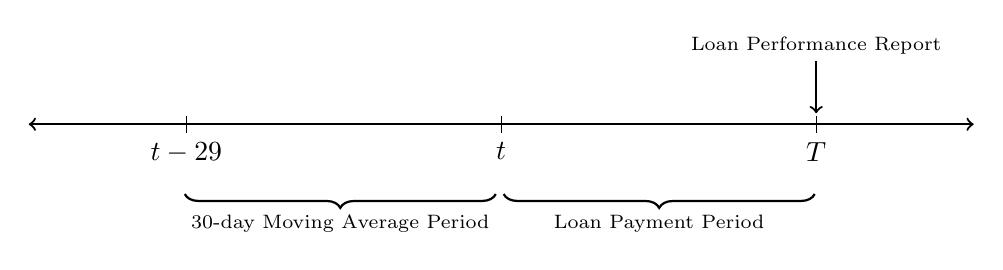
\begin{tikzpicture}
        % draw horizontal line   
            \draw[thick, <->] (0,0) -- (12,0);
            % draw vertical lines
            \foreach \x in {2,6,10}
            \draw (\x cm,3pt) -- (\x cm,-3pt);
        
            \draw[ultra thick] (2,0)  node[below=3pt,thick] {$t-29$} node[above=3pt] {};
            \draw[ultra thick] (6,0)  node[below=3pt,thick] {$t$}    node[above=3pt] {};
            \draw[ultra thick] (10,0) node[below=3pt,thick] {$T$}   node[above=3pt] {};
        
               \draw [ black, thick,decorate,decoration={brace,amplitude=5pt},
               xshift=8pt,yshift=-11pt] (9.7,-0.5) -- (5.75,-0.5)
               node [black,midway,below=4pt,xshift=0pt] {\scriptsize Loan Payment Period};
        
               \draw [ black, thick,decorate,decoration={brace,amplitude=5pt},
               xshift=8pt,yshift=-11pt] (5.65,-0.5) -- (1.7,-0.5)
               node [black,midway,below=4pt,xshift=0pt] {\scriptsize 30-day Moving Average Period};
                
               \draw [thick,->, ] (10,0.8) -- (10,0.14);
               \node[align=center] at (10,1.0) {\scriptsize Loan Performance Report};
              
        \end{tikzpicture}
        \end{center}
        
 In the diagram, $t$ represents the reporting period beginning date of a particular security ABS-EE filing and $T$ is the reporting period ending date. The time span $T-t$ is roughly 30-days (1 month) for all loans in the sample. A moving average is constructed for a total of 30 days by considering the 29 days proceeding a reporting period start date and the day the reporting period begins, which corresponds to the time span from $t-29$ to $t$. The calculated average is a simple moving average which implies each day's measure is weighted by the number of periods in the average, i.e. a weight of $1/30$ for each day. This choice of average was selected for its simplicity, but it is possible that a weighted moving average could also have been a reasonable option, where days that are closer to a reporting period beginning date are given a higher weight.   With this framework, mobility measures can be generated for each loan in the sample by date and county. Concretely, the formula used to generate the moving-average would be the following:
        \begin{equation}
        M_{t,c} = \frac{1}{30} \sum_{i=0}^{29} \frac{T_{t-i,c}}{P_{c}} \times 100
        \end{equation}
        \begin{center}\begin{tabular}{lll}
        $M_{t,c}$ & \sim & 30-day moving average of mobility in time $t$ and county $c$ \\
        $T_{t-i,c}$ & \sim & Daily count of trips $\geq$25 miles in time $t-i$ and county $c$ \\
        ${P_{c}}$ & \sim & Census Bureau population estimate for county $c$ in 2019 \vspace{0.3em} \\
        \end{tabular}\end{center}
To illustrate how the moving average measure corresponds to daily variation in mobility\hypertarget{Trips Fig Back}, see the following example figure that overlays the variables overtime for New York County, NY:\footnote{New York County is a populous county that largely encapsulates the Manhattan borough of NYC and some other surrounding area. Many large commercial enterprises are located there.}
\begin{equation*}
        \text{[ \hyperlink{Trips Fig}{Figure 7}: Mobility Overtime (New York County, NY) ]}
\end{equation*}
From this figure, the volatility of the mobility measure (blue line) is very clear. The overlayed 30 day average appears to fit the overall trend well and is less affected by drastic short term spikes or dips. \hyperlink{Summary Statistics}{Table 1} in Section 8.2 also provides summary statistics for mobility within the sample. The average value is about 21.1 and median is 19.7, which would imply about 1 in 5 people within a county make a $\geq$25 mile trip each day. This appears to be a reasonable approximation considering that individuals who are not actively working and commuting, like small children and the elderly, would probably not be making routine trips of this length. 
  
\subsection{PPP and EIDL Activity}
This paper seeks to employ a dual perspective on the impacts of government aid by evaluating both PPP and EIDL activity during the pandemic. Two measures are constructed for each program to capture the magnitude \textit{and} spread of loan uptake. Each are calculated on a daily basis since the programs were implemented in early April 2020. The first is \textit{Funding Coverage} (\textit{FCov}) and is intended to measure the magnitude of loan aid within a county at a given time. It is calculated as the following:
\begin{equation}
    FCov_{t,c} = ln\left[1 + \frac{1}{B_{c}}\sum_{i=\tau}^{t}F_{t,c}\right]
\end{equation}
        \begin{center}\begin{tabular}{lll}
        $FCov_{t,c}$ & \sim & Natural log of cumulative PPP (or EIDL) funding per business in time $t$ and \\
        $ $ &  & county $c$ business at time $t$ in county $c$ \\
        $F_{i,c}$ & \sim &  Cumulative PPP (or EIDL) funds at time $t$ in county $c$ \\
        ${B_{c}}$ & \sim & BLS total business count in county $c$ from Q1 2020 \\
        \end{tabular}\end{center}
The time period $\tau$ represents the first day the program officially opened for loan approval on April 3\textsuperscript{rd}, 2020. The natural log of the ratio is taken such that marginal increases in regression analysis can be interpreted as a ``percent change in funding coverage" or a ``percent change in funding per business."\footnote{An additional +1 (or \$1) is added such that the measure does not equal \$0 in instances when a county received no funding. This is a very minor adjustment to address the fact that observations must strictly be $\geq$1  for the natural log to be defined and non-negative.} The second measure is \textit{Loan Coverage} (\textit{LCov}) which can address some potential shortfalls with only considering funding coverage in analysis. In particular, funding coverage could produce a similar result if many small businesses in county were approved for a number of small loans or one business received a considerably large loan. Moreover, the ratio in isolation does not provide some useful information about how loans were dispersed within a county. Thus, considering funding coverage is useful to address the \textit{spread} of PPP funding, not just magnitude. Concretely, the formula for loan coverage would be:
\begin{equation}
    LCov_{t,c} = \frac{1}{B_{c}}\sum_{i=\tau}^{t}\L_{i,c} \times 100
\end{equation}
        \begin{center}\begin{tabular}{lll}
        $LCov_{t,c}$ & \sim & Cumulative PPP (or EIDL) loans per business ($\times$ 100) in time $t$ and county $c$ \\
        $L_{t,c}$ & \sim &  Cumulative PPP  loans at time $t$ and county $c$ \\
        ${B_{c}}$ & \sim & BLS total business count in county $c$ from Q1 2020 \\
        \end{tabular}\end{center}

Literature that utilizes PPP origination data have proposed a variety of options for measuring its impact on a particular area. \hyperlink{Agarwal}{Agarwal, et al.} (2021) implement this paper's measure for PPP loan coverage, which is the ratio of cumulative PPP loans received in a county divided by the number of businesses in the county at a given point in time. Moreover, they focus on the program's spread rather than magnitude. \hyperlink{Li}{Li \& Strahan} (2020) also create their own measure that uses businesses specifically larger than 500 employees as a denominator, with estimates provided by County Business Patterns data released by the BLS. Defining a measure to address business size is certainly a relevant consideration but is not addressed in this paper for the following two reasons. The first is that most counties are composed of +99\% businesses that have 500 employees or less. The second reason is that the SBA's actual thresholds concerning business size are quite complicated and flexible in reality. Size standards can vary significantly based on industry, total revenue, or many other factors. Firms also have different options for calculating their size and current number of employees, which could add yet another layer of complexity about determining which are eligible. Given all this, it seems logical that total businesses can be a reasonable proxy for business presence even through it does not perfectly address more subtle rules concerning business eligibility. Overall, employing two measures for both loan programs could be a useful contribution to COVID-19 literature; a singular focus on a program's spread or magnitude might be too narrow a perspective and ultimately could omit important characteristics of fund allocation.

\hyperlink{Summary Statistics}{Table 1} in Section 8.2 provides summary statistics for both programs uptake measures. Within the sample, average funding coverage for PPP and EIDL was about \$56,700 and \$17,450, respectively. In the most extreme case, it appears that loan coverage for each program can exceed 100\%, which implies a higher number of loans than businesses within a county. This result is not unreasonable considering that some slight discrepancies could arise from using business count estimates from BLS and also having zip codes of loans mapped (approximately) to the county-level.\footnote{For clarification, see again \hyperlink{Commercial Mortgage Performance}{Section 4.1} that describes how mapping zip codes to county FIPS was handled using population densities.} The fact that average loan coverage is roughly 50\% with a county points to the widespread business demand for PPP loans during the pandemic. Average loan coverage of 32\% for EIDL illustrates its large scope as well.  

\subsection{Econometric Model}
To investigate how commercial mortgage distress affected by government aid and mobility during the pandemic, this paper employs a fixed effects framework (FE) at the loan-level for analysis. FE has been a popular choice for researchers operating with panel data and investigating the effects of the pandemic overtime and across the country (\hyperlink{Autor}{Autor, et al.} 2020, \hyperlink{Granja}{Granja, et al.} 2020, \hyperlink{Hubbard}{Hubbard \& Strain} 2020, \hyperlink{Li}{Li \& Strahan} 2020). The de-meaning process of FE is useful to effectively control for many aspects of loan heterogeneity at origination and many other time-invariant attributes across CMBS, where securities often have different underwriters, servicers, and originators.\footnote{Examples of loan characteristics could be: interest rate, loan amount, term, maturity date, original LTV, a ballon payment indicator, and many others.} \hyperlink{Agarwal}{Agarwal et al.} (2020) also emphasize that loan fixed effects rule out local tendencies or regulations that often can be influential factors in deterring mortgage default.

To address within-loan correlations overtime, standard errors are clustered at the loan-level within every model. Year-month fixed effects are also included in all regressions to control for that common economic and pandemic-related trends over the course of the sample.\footnote{More specifically, time fixed effects would effectively eliminate omitted variable bias for factors that vary overtime, but are constant across entities. For example, this could be CDC or Federal policies that would apply to businesses and individuals across the country.} Formally\hypertarget{Regression}, the FE regression specification is the following:
\begin{equation}
    Y_{i,t,c} = \kappa + \beta L_{t,c}  + \lambda(M_{t,c}\times Covid) + \theta M_{t,c} + \phi U_{t,c} + \delta C_{i,t,c} + \alpha_i + \tau_t + \epsilon_{i, t, c}
\end{equation}
\begin{center}\begin{tabular}{lll}
$Y_{i,c,t}$ & \sim & Binary indicator variable for loan distress for a loan $i$ in time $t$ and county $c$ \\
$L_{i,t,c}$ & \sim & Matrix of PPP and EIDL activity measures in time $t$ and county $c$ \\
$M_{t,c}\times Covid$ &\sim& Mobility and COVID-19 period interaction term \\
$M_{t, c}$ & \sim & Mobility measure at time $t$ and county $c$ \\
$U_{t,c}$ & \sim & One-month lagged unemployment rate at time $t$ and county $c$ \\
$C_{i,t,c}$ & \sim & Matrix of time-variant loan characteristics for loan $i$ at time $t$ and county $c$ \\
$\alpha_{i}$ &\sim& Loan-level fixed effects \\
$\tau_{t}$ &\sim& Time (year-month) fixed effects \\
$\epsilon_{i,t, c}$ & \sim & Error term \vspace{0.4em}
\end{tabular}\end{center}

The dependent variable $Y_{i,t,c}$ represents one of the three measures of mortgage distress described in \hyperlink{Defining Commercial Mortgage Distress}{Section 5.1}, specifically: default ($\mathbb{D}$), special servicing ($\mathbb{S}$), or delinquency transition ($\mathbb{T}$). Since these variables are binary, the marginal effects within the model can be interpreted as changes in probability, or likelihood, of distress. $L_{t,c}$ is the matrix of government aid variables which are expected to be inversely related to loan distress. The interaction term $M_{t,c}\times Covid$ is the main variable of focus to determine the effect of mobility on loan distress, conditional on the time period being the COVID-19 pandemic.\footnote{Specifically, the COVID-19 period within analysis is defined as any reporting period starting from April 1\textsuperscript{st}, 2020 and afterwards. This enables lagged shifts in independent variables that occurred when the pandemic began in March to be considered part of the pandemic period, which would have affected loan payments during April.} Considering mobility as a proxy for consumer and supplier activity, it is expected that a higher measure during the pandemic will reduce likelihood of distress, i.e. produce a negative coefficient. However, it is unclear if a result would be economically significant, especially after considering other relevant controls within the model.

$C_{i,t,c}$ is a matrix of time-variant loan characteristics, that were outlined in \hyperlink{Time-Variant}{Section 5.2}: remaining term, most recent DSCR, and most recent occupancy. The expected effect for a loan's remaining term is somewhat ambiguous. It is arguable that more seasoned loans, i.e. a shorter remaining term, indicate experienced and financially stable borrowers. Nevertheless, it is also possible that newer borrowers have more robust emergency reserves available, making them more resilient during an economic shock. Both most recent DSCR and occupancy are expected to be inversely associated with probability of distress. Higher DSCR indicates strong free cash flow relative to mandatory debt payments, a clear signal of financial stability and larger cushion against a business disruption. Increased occupancy most likely corresponds to high demand for rentals, which also implies stronger cash flow. Lagged unemployment, a time-variant characteristic at the county-level, is included as $U_{t,c}$ and is added as another relevant factor to address contemporaneous economic conditions between counties. As a benchmark indicator of economic downturn, it is expected to be positively correlated with loan distress. 

\hyperlink{Regression}{Equation (4)} is estimated for the entire sample of roughly 5,900 loans and then across each of the six individual property types: retail, office, lodging, mixed-used, multi-family, and industrial. While the model selection aligns well with prevailing literature, there are many possible ways that it could be potentially improved and/or expanded, such as adding additional time-variant loan characteristics or county-level government policies. Using a larger sample of loans, \hyperlink{Agarwal}{Agarwal et al.} (2020) also added a variable to capture average delinquency of neighboring commercial mortgages within a county, presumably investigating spillover effects of financial distress. More details on these types of considerations will be discussed again in the concluding remarks about future research, specifically \hyperlink{Future Research Considerations}{Section 7.3}. See the next section for a complete discussion of empirical results that are presented in \hyperlink{Empirical Results Tables}{Section 9}\hypertarget{Empirical Results}. 

% https://www.youtube.com/watch?v=L9ZL6_DB4fQ
% http://www.cazaar.com/ta/econ113/interpreting-beta

\section{Results}
The results for estimating \hyperlink{Regression}{Equation (4)} on the different measures of loan distress are discussed in detail below. Regression tables are formally presented in \hyperlink{Empirical Results Tables}{Section 9}. In each table, coefficient t-statistics are reported in parentheses, which are calculated from robust standard errors clustered at the loan-level. Given each dependent variable is a binary indicator equal to 1 if a loan satisfied certain criteria for being distressed, a positive coefficient in the model implies increased probability of loan distress, and vice versa. Within the models, all coefficients also represent the marginal effect of a unit (+1) increase in the independent variable. For the most part, this effect is a percentage point ($pp$) increase in the dependent variable, which is important to distinguish from a percent increase (\%)\hypertarget{Regression 1 Back}.\footnote{Percentage changes refer to $\Delta$DV / Mean of DV (DV = Dependent Variable).} Both types of effects are reported, where percentage increases are usually given in parentheses. 

There are some instances where a unit-increase in an independent variable is not a percentage point increase. For PPP and EIDL Funding Coverage, which are both ratios transformed using the natural log, a unit-increase is interpreted as a percentage increase (not percentage point) in funding coverage or ``funding per business." The measure for Most Recent DSCR can be intuitively thought of as a property's net operating income as a multiple of debt service, where a value of 2.0 is 2.0x debt service or 200\% larger. Accordingly, a unit increase in DSCR should be interpreted as a +100 percentage point increase. It is also important to note that unique considerations are made to report the marginal effects of the interaction term between mobility and COVID-19. For this term, a percentage change is reported by dividing a given coefficient by \textit{pre-pandemic} average loan distress. For additional clarification on how all marginal effects were determined, see \hyperlink{Marginal Effects}{Section 12.3} of the Appendix. 

\subsection{Aggregate Sample}
\hyperlink{Regression 1}{Table 2} shows empirical results for each type of distress measure using the full sample of commercial mortgages. For each distress measure, a model is estimated with and without time-variant loan characteristics, illustrating the relevance of these characteristics in most regressions and the overall robustness of other results.\footnote{For example, see that Column (1) and Column (2) both feature default ($\mathbb{D}$) as the dependent variable. In Column (2), the three time-varying loan characteristics are added to the model. This approach is the same for the subsequent columns.} At the top of each column, the type of distress is also indicated with its bold-lettered notation.

With default ($\mathbb{D}$) as the dependent variable in Column (2), the contrasting effects of government aid programs are evident. Coefficients for PPP funding and loan coverage are both significant at the 1\% level. A percent increase in PPP funding per business corresponds to a +0.016\hspace{0.20em}$pp$ (+0.52\%) in likelihood of default. With PPP loan coverage, a percentage point increase implies +0.075\hspace{0.20em}$pp$ (+2.4\%) higher likelihood of default.\footnote{The average for default in the regression model was 3.12\%.} This is the one instance suggesting uptake for PPP was higher in areas where commercial businesses were more adversely affected by the pandemic. In contrast, increases in EIDL funding and loan coverage are associated with -0.0043\hspace{0.20em}$pp$ (-0.14\%) and -0.03\hspace{0.20em}$pp$ (-1.03\%) reductions in likelihood of default, respectively. This result supplements literature, such as \hyperlink{Fairlie}{Fairlie \& Fossen} (2020), that finds some beneficial effects from EIDL during the pandemic. With both programs, the economic significance of magnitude of loan coverage appears more substantial than loan spread. With the mobility interaction term in Column (2), it is also evident that a percentage point increase corresponds to a -0.12\hspace{0.20em}$pp$ lower likelihood of default, a result significant at the 1\% level. When comparing this marginal effect to average default in the sample before the pandemic began, this implies a sizable -35.6\% decrease in probability of default. Considering local economic conditions, higher county-level unemployment raises likelihood of default by 0.12\%\hspace{0.20em}$pp$ (+3.8\%). Measures for DSCR and occupancy are also highly significant at the 1\% level, and as expected, an increase in either is inversely related to probability of default. 

Now considering Column (4) with special servicing ($\mathbb{S}$) as the dependent variable, loan coverage is the one aspect of the PPP that is statistically significant. The likelihood of a special service increases by 0.08\hspace{0.20em}$pp$ (+2.6\%) for a percentage point increase in PPP loan coverage. This effect is very similar to what was found in Column (2). Both measures for EIDL have negative coefficients but are not statistically significant. One potential reason why no result was found with either EIDL variable could be attributed to the notion that is a more subjective indicator of distress than default or delinquency transition, so its association with government aid uptake could be less apparent. It is quite possible that many loans transferred to special servicers remained current and financially stable, i.e. the transfer was only an act of precaution by the master servicer. The variable of focus for mobility is found to be significant at the 1\% level where a percentage point increase in the interaction term is associated with a -0.10\hspace{0.20em}$pp$ (-30.5\%) decrease in likelihood of special service. All time variant loan characteristics correspond with decreased probability of special service, where Loan Remaining Term is marginally significant.\footnote{The reported coefficient had a t-statistic of 1.94.}

Finally, Column (6) features delinquency transition ($\mathbb{T}$) as the dependent variable. Similar to Columns (2) and (4), PPP Funding Coverage is found to be positively associated with loan distress, significant at the 1\% level. A percentage increase in Funding Coverage is associated with +0.013\hspace{0.20em}$pp$ (+0.41\%) higher likelihood of a transition. One possible explanation for this result is that the bulk of PPP funding was being approved in April -- May 2020, when CRE distress also began to accelerate. Similar to Column (2), the result suggests that PPP funding flowed to places where signs of distress within CRE are more apparent. The interaction term for mobility during the pandemic has a negative coefficient and statistically significant at the 5\% level, illustrating the robustness of this result across various measures of distress. A percentage point increase in the interaction corresponds to a -0.04\hspace{0.20em}$pp$ (-12.9\%) in likelihood of transition\hypertarget{Regression 2 Back}. County-level unemployment is also found to have a positive association with delinquency transition. Coefficients for time-varying loan characteristics are similar to the past two models, albeit with less statistical significance in the case of Most Recent DSCR. 

\subsection{Property Heterogeneity}

\subsubsection{Default}
Regression estimates in \hyperlink{Regression 2}{Table 3} analyzes probability of default ($\mathbb{D}$) across each property type. Similar to results in aggregate, the effect of the PPP Funding Coverage seems to indicate higher likelihood of default where it is statistically significant. In particular, for retail and lodging, a percent increase in PPP Funding Coverage is associated with increases of +0.03\hspace{0.20em}$pp$ (+1.37\%) and +0.17\hspace{0.20em}$pp$ (+1.63\%) in probability of default, respectively. There is also a marginally significant result for mixed-use properties of +0.03\hspace{0.20em}$pp$ (+0.85\%).\footnote{The reported t-statistic for the coefficient on PPP Funding Coverage for mixed-use was 1.90.} PPP Loan Coverage is only found to be impactful for multi-family property with a coefficient of +0.12\hspace{0.20em}$pp$ (+7.3\%). These results contrast somewhat with \hyperlink{Agarwal}{Agarwal et al.} (2020), that found negative effects for loan coverage, particularly for smaller sized mortgages.\footnote{It is important to note that \hyperlink{Agarwal}{Agarwal et al.} (2020) did not also consider funding within their model specifications.} They also did not find any connection between their measures PPP loan coverage, default, and small-sized lodging mortgages. Effects found for EIDL were only apparent for multi-family properties as well. Notably, a percent increase in EIDL Funding Coverage can be seen to reduce default probability by -0.007\hspace{0.20em}$pp$ (-0.45\%). 

Mobility during the pandemic is found to be a significant factor in reducing likelihood of default within office, lodging, and multi-family properties.\footnote{There is an additional, marginally significant result for office space with a reported t-statistic of 1.74.} Specifically, a percentage point increase reduces likelihood of default in a given month by -0.07\hspace{0.20em}$pp$ (-56.5\%), -0.36\hspace{0.20em}$pp$ (-67.3\%), and -0.17\hspace{0.20em}$pp$ (-35.1\%), respectively. These results for mobility during the pandemic also appear contrast pre-pandemic coefficients, which are largely insignificant or positive and marginally significant in some cases. As expected, unemployment rates are impactful across different property types, notably retail, lodging, and mixed-use. With time-variant loan characteristics, the only non-intuitive finding is that higher DSCR is associated with increased likelihood of distress for lodging properties. This might be attributable to the fact that even hotels with strong cash flow were not insulated well from the sharp drop in travel, both domestically and internationally. Additionally, it appears that the sample of industrial properties has no significantly robust results. This is not completely unexpected considering that distress caused by the pandemic for this property type has been relatively tame\hypertarget{Regression 3 Back}. 

\subsubsection{Special Servicing}
\hyperlink{Regression 3}{Table 4} focuses on special servicing ($\mathbb{S}$) as a dependent variable within each property-level regression model. Results for PPP Funding Coverage are relatively similar to the previous table for retail and lodging, which both have coefficients significant at the 1\% level. For these two property types, a percentage increase in PPP Funding Coverage raises probability of special service by +0.016\hspace{0.20em}$pp$ (+0.70\%) and  +0.13\hspace{0.20em}$pp$ (+1.21\%). The results of the PPP are marginally significant and mixed for office space. While a negative coefficient for PPP Funding Coverage in Column (2) does suggest a positive effect of the PPP, this result is nuanced by a positive coefficient for PPP Loan Coverage.\footnote{Reported t-statistics for PPP Funding Coverage and PPP Loan Coverage for office property were -1.85 and 1.96, respectively.} Moreover, it does not appear there is any one-sided evidence regarding a benefit of the PPP for a particular property type in analysis thus far. For EIDL, the single statistically significant result is found for Funding Coverage and office property. Specifically, a percentage increase in EIDL Funding Coverage corresponds to a decrease of -0.001\hspace{0.20em}$pp$ (-0.28\%) in likelihood of special service. 

A robust, distress-reducing effect was found for the mobility interaction term and lodging in Column (3), where a percentage point increase lowers likelihood of special service by -0.33\hspace{0.20em}$pp$ (-62.8\%). Other results, significant at the 10\% level, were found with retail and office space.\footnote{Note that the reported t-statistics for retail and office in this case were -1.94 and -1.85.} Local travel has proven an economically meaningful determinant of loan distress for lodging properties thus far, and there do not appear to be any statistically significant instances where the mobility interaction term raises likelihood of distress. County-level unemployment has a statistically significant coefficient for lodging and multi-family properties. This is another variable that has had positive and robust results for lodging properties in particular\hypertarget{Regression 4 Back}. Notable results for time-variant loan characteristics indicate that lower DSCR corresponds to higher likelihood of special service for retail properties. 


\subsubsection{Delinquency Transition}
\hyperlink{Regression 4}{Table 5} illustrates the last series of property-level regressions, where delinquency transition ($\mathbb{T}$) is the dependent variable. Like in the previous two tables, higher PPP Funding Coverage at the county-level raises likelihood of distress for lodging properties, a result that is significant at the 1\% level. In Column (3), a percentage increase in PPP Funding Coverage is associated with a +0.083\hspace{0.20em}$pp$ (+0.78\%) increase in likelihood of a transition. Column (1) for retail also shows a marginally significant, positive coefficient for PPP Funding Coverage. For multi-family property in Column (4), there are contrasting effects for the PPP. The coefficient for PPP Funding Coverage is negative and statistically significant at the 5\% level, giving one indication that PPP uptake was associated with lower likelihood of transition. However, there is also a marginally significant result for PPP Loan Coverage in Column (4) that nuances the overall effect of the PPP in this case. For EIDL uptake, it can be seen that there is also a marginally significant result suggesting that higher Loan Coverage reduces likelihood of transition for multi-family properties. 

Coefficients for the mobility interaction term were negative and significant at the 5\% level for retail and mixed-use property. A percentage point increase corresponded to -0.058\hspace{0.20em}$pp$ (-18.0\%) and -0.19\hspace{0.20em}$pp$ (-111.5\%) decreases in likelihood of transition, respectively. Thus, across different measures of distress and property types, the impact of mobility during the pandemic has been either risk-reducing or insignificant. A percentage point increaes in county-level unemployment is found to increase likelihood of transition by -0.12\hspace{0.20em}$pp$ (+5.38\%). For time-variant loan characteristics, the most significant result was a unit-increase (+100\hspace{0.20em}$pp$) in Most Recent DSCR corresponding to a -1.15\hspace{0.20em}$pp$ (-10.8\%) in the probability of delinquency transition for lodging properties\hypertarget{Conclusion}. Very little significant results were found for industrial space, which again could be attributed to its apparent stability during the pandemic. 


\section{Conclusion}

\subsection{Synopsis}

The financial stability of commercial real estate (CRE) has been upended by the COVID-19 pandemic. Delinquency rates across many different property types have surged and show limited signs of recovery for over a year after virus arrived in the United States. Research focused on this extensive market is vital considering the risks of deteriorated commercial mortgage performance and its association with an unprecedented degree of federal stimulus. 

This paper investigated how financial distress of commercial mortgages was 
affected by government aid and mobility during the pandemic. While many papers have focused on the Paycheck Protection Program (PPP) since its inception in April 2020, this paper sought to supplement prevailing literature by employing a dual perspective on government aid. It evaluated the PPP and Economic Injury Disaster Loans (EIDL) simultaneously in analysis, bridging a connection between the two programs. This paper also focuses on changes in loan performance due to government aid, rather than employment levels, which could be a valuable perspective to add for a comprehensive review of each program by policymakers. The paper's second focus on mobility as a determinant of loan distress quantitatively addresses the question of how important local travel is to the financial health of CRE during the pandemic, where there is considerable heterogeneity of policy action and health intervention across the country.

Data for analysis was sourced from a variety of public sources, namely \href{https://finsight.com/}{Finsight}, the \href{https://www.sba.gov/}{SBA}, and the \href{https://www.bts.gov/}{BTS}. A fixed effects model was then employed over the time period Jan. 2019 -- Feb. 2021 to determine if there were any economically and statistically significant effects. Results found indicated there was a positive relationship between measures of PPP uptake and loan distress, which could suggest that PPP funds flowed to areas adversely by the pandemic. Findings did not indicate that PPP activity in a county corresponded to reduced likelihood of loan distress for commercial mortgages in the area. When considering EIDL, results predominantly indicated a benefit of the program, especially in cases of distress derived from loan delinquencies. Mobility from the pandemic was found to be largely distress-reducing, especially for lodging properties. Other findings for county-level unemployment and time-variant loan characteristics could also prove informative for monitoring CRE credit risk and the larger economic recovery from COVID-19. 

\subsection{Policy Implications}

A comprehensive review of the PPP should be paramount to policymakers given its novel purpose, size, and scope. Accordingly, a focus on the program's impact on CRE is a valuable alternative perspective to have when making considerations about future funding allocation and for deciding the ultimate success of the program. Considering that the program is active as of April 2021, the latter is not possible to infer from this paper's findings, but the methodology could be a useful framework to re-implement in the future when the PPP expires. Results provide some positive evidence to policymakers that funding and loan coverage is finding its way to hard-hit areas of the pandemic, but the actual benefits could not be reaching large commercial mortgages. This might inform policymakers that commercial mortgages, especially conduit loans from private-label securities, could be deserving of more targeted aid. The Federal Reserve has implemented some CMBS asset-purchasing to support market liquidity, but private-label securities are not included. That aid had been allocated to agency-CMBS and mainly multi-family space rather than nonresidential property (\hyperlink{Scott}{Scott} (2020[1]).\footnote{Also see the Fed FAQ on CMBS purchases \href{https://www.newyorkfed.org/markets/domestic-market-operations/monetary-policy-implementation/agency-commercial-mortgage-backed-securities/agency-commercial-mortgage-backed-securities-faq}{here} from March 17\textsuperscript{th}, 2021.} 

This paper illuminated potential benefits of the EIDL for policymakers and could be the first piece of literature to investigate a connection between the program and CRE during the pandemic. EIDL was smaller than the PPP but should not be overlooked within academic research on government aid during the pandemic. In 2021, the maximum loan size for EIDL is also being raised, which make it even more potent an option for large commercial mortgage borrowers. Similar to the PPP, when EIDL has fully expired, this paper's methodology could be re-applied for a more conclusive determination on the success of the program. Findings indicating benefits could be most pertinent in the present to policymakers who are trying to decide whether or not to add more fund allocation or extend the program further into 2021. More generally, this paper could also serve as a caution to policymakers by drawing some additional attention to the current the long-term future of CRE, which the pandemic has shrouded in uncertainty. Even when health interventions and government policies largely recede, serious financial risk could remain in this industry due to an accelerated shift away from ``brick-and-mortar" establishments by consumers and lessees (\hyperlink{Grant}{Grant} 2020, \hyperlink{Putzier}{Putzier} 2020). Retail, mixed-use, and even office space, which has been more relatively more resilient during the pandemic, could face downward pressure on occupancy levels and property values. This could increase the urgency to have more government aid available for CRE.

Beyond government policy specifically, findings also have possible applications with private-sector policy for CRE risk management and portfolio allocation. Those concerned with determining early indicators of loan distress might find measures of government a viable option in this context. Even if PPP funding in a county did not benefit commercial mortgages, it did show a strong association with higher distress likelihood, which could help indicate where credit risk is mounting. Monitoring county-level shifts in mobility could have similar benefits for risk management. Other results related to unemployment, DSCR, and occupancy levels help to confirm conventional insights in financial literature about each being key credit risk metrics. 


\subsection{Future Research Considerations}

There are many considerations for future research that could improve the validity, scope, and robustness of this paper's results. Perhaps most importantly, the conclusivity of findings are limited by the fact that the COVID-19 pandemic is ongoing in early 2021. Re-implementing the methodology in the future is recommended, especially when the PPP and EIDL have both been closed. Given that all data sources are publicly accessible, and CMBS reporting is updated monthly on \href{https://finsight.com/}{Finsight}, keeping the research focus active is certainly not unrealistic and could provide timely insights as the status of CRE continues to evolve rapidly. 

The methodology of this paper could be refined in regard to selecting data, variables, and an econometric model. While the commercial mortgage data from CMBS ABS-EE files was granular, it is restricted to a recent post-2016 timeframe and did not include any pre-2008 origination, i.e. CMBS 1.0. Combining this data with additional loans and securities with older origination could produce a more comprehensive sample of the current U.S. commercial mortgage industry. There are also many other property types, beyond the six analyzed in this paper, that could be added in future research, such as: cooperative housing, self-storage, and health-care.\footnote{Within ABS-EE files, data on these property types was relatively sparse. However, other commercial mortgage data providers, such as \href{https://www.trepp.com/}{Trepp}, could potentially have more variety.} Having other time-variant loan characteristics could improve the robustness of results, such as: loan-to-value (LTV) ratio or current interest rate.\footnote{\hyperlink{Agarwal}{Agarwal, et al.} (2021) is one example where these variables were added and produced impactful results.} In addition to unemployment rates, county-level controls for economic conditions, such as local government policies, could be added as the data becomes available from other researchers (\hyperlink{Spiegel}{Spiegel \& Tookes} 2020, \hyperlink{Golsbee}{Golsbee et al.} 2020). There are many options that could bolster evaluation of government aid. New variables for PPP and EIDL could be generated, like the degree of aid by different NAICs code.\footnote{A stratification by NAICs sector would be possible the PPP at this time. A variable for NAICs code is not included within EIDL data, but could be added by the SBA in future data updates.} Having analysis broken down by various funding rounds, would also build further on the work of \hyperlink{Agarwal}{Agarwal, et al.} (2021), \hyperlink{Granja}{Granja, et al.} (2020), and many others. Other model choices, like event-study frameworks focused on heterogeneity of conditions across different state-lines (\hyperlink{Spiegel}{Spiegel \& Tookes} 2020), could prove useful in determining the robustness of results. These considerations, and possibly many others, applied to future research will facilitate a better understanding of the consequences of the COVID-19 pandemic for commercial real estate, in turn helping to shape optimal economic policy moving forward. 

\newpage

% \section{Citation List}
% \hyperlink{Agarwal}{Agarwal, et al.} (2021)         \\ 
% \hyperlink{Chetty}{Chetty, et al.} (2020)            \\ 
% \hyperlink{Agostino}{Agostino, et al.} (2020)        \\
% \hyperlink{Autor}{Autor, et al.} (2020)             \\
% \hyperlink{Alekseev}{Alekseev, et al.} (2020)        \\ 
% \hyperlink{Barrios}{Barrios, et al.}  (2020)        \\
% \hyperlink{Barrot}{Barrot, et al.} (2020)           \\ 
% \hyperlink{Bachas}{Bachas, et al.} (2020)           \\
% \hyperlink{Fabozzi}{Fabozzi} (2005)                 \\
% \hyperlink{Li}{Li \& Strahan} (2020)                 \\
% \hyperlink{Santos}{Santos} (2020)                    \\
% \hyperlink{AJMC}{AJMC} (2021)                        \\
% \hyperlink{Hubbard}{Hubbard \& Strain} 2020
% \hyperlink{Granja}{Granja, et al.} (2020)           \\ \\ \\ \\

% \noindent
% (\hyperlink{Agarwal}{Agarwal, et al.} 2021)                 \\ 
% (\hyperlink{Chetty}{Chetty, et al.} 2020)                   \\ 
% (\hyperlink{Agostino}{Agostino, et al.} 2020)               \\
% (\hyperlink{Autor}{Autor, et al.} 2020)                    \\
% (\hyperlink{Alekseev}{Alekseev, et al.} 2020)               \\
% (\hyperlink{Santos}{Santos} 2020)                          \\ 
% (\hyperlink{Barrios}{Barrios, et al.}  2020)               \\
% (\hyperlink{Barrot}{Barrot, et al.} 2020)                   \\ 
% (\hyperlink{Bachas}{Bachas, et al.} 2020)                   \\
% (\hyperlink{Fabozzi}{Fabozzi} 2005)                         \\
% (\hyperlink{Li}{Li \& Strahan} 2020)                        \\
% (\hyperlink{AJMC}{AJMC} 2021)                             \\
% (\hyperlink{Granja}{Granja, et al.} 2020)                   \\


\newpage
\thispagestyle{plain}
\clearpage
\phantomsection
\newgeometry{margin=1.00in,top=0.50in,bottom=1.0in}
\tiny{\textcolor{white}{}}\hypertarget{References}\tiny{\text{}}
\normalsize
\addcontentsline{toc}{section}{References}

\begin{thebibliography}{40}

\bibitem{Agarwal}
\hypertarget{Agarwal}
Agarwal, Ambrose, Lopez, and Xiao (2021) ``Did the Paycheck Protection Program Help Small Businesses? Evidence from Commercial Mortgage-Backed Securities,"  Available at SSRN:\\ \href{ https://ssrn.com/abstract=3674960}{https://ssrn.com/abstract=3674960} or \href{http://dx.doi.org/10.2139/ssrn.3674960}{http://dx.doi.org/10.2139/ssrn.3674960}

\bibitem{AJMC}
\hypertarget{AJMC}
American Journal of Managed Care, or AJMC (2021) ``A Timeline of COVID-19 Developments in 2020," Last updated January 1\textsuperscript{st}, 2020. Available at: \href{https://www.ajmc.com/view/a-timeline-of-covid19-developments-in-2020}{https://www.ajmc.com/view/}

\bibitem{Alekseev}
\hypertarget{Alekseev}
Alekseev, Amer, Gopal, Kuchler, Schneider, Stroebel, \& Wernerfelt (2020) ``The Effects of COVID-19 on U.S. Small Businesses: Evidence from Owners, Managers, and Employees," \textit{Working Paper 27833.} Available at: \href{http://www.nber.org/papers/w27833}{http://www.nber.org/papers/w27833}

\bibitem{Autor}
\hypertarget{Autor}
Autor, Cho, Crane, Goldar, Lutz, Montes, Peterman, Ratner, Villar, \& Yildirmaz (2020) ``An Evaluation of the Paycheck Protection Program Using Administative Payroll Microdata," \textit{Preliminary} version as of July 22\textsuperscript{nd}, 2020. Available at: \href{http://economics.mit.edu/files/20094}{http://economics.mit.edu/files/20094} 

\bibitem{Bachas}
\hypertarget{Bachas}
Bachas, Ganong, Noel, Vavra, Wong, Farrel, \& Greig (2020) ``Initial Impacts of the Pandemic on Consumer Behavior: Evidence from Linked Income, Spending, and Savings Data," NBER Working Paper \#27617. Available at: \href{https://www.nber.org/papers/w27617}{https://www.nber.org/papers/w27617}  

\bibitem{Baker}
\hypertarget{Baker}
Baker, Farrokhinia, Meyer, Pagel, Yannelis (2020) ``How Does Household Spending Respond to an Epidemic? Consumption during the 2020 COVID-19 Pandemic," NBER Working Paper \#26949. Available at: \href{https://www.nber.org/papers/w26949}{https://www.nber.org/papers/w26949}

\bibitem{Barrios}
\hypertarget{Barrios}
Barrios, Minnis, Minnis, \& Sijthoff (2020) ``Assessing the Payroll Protection Program: A Framework and Preliminary Results,"  Available at SSRN: \\ \href{https://ssrn.com/abstract=3600595}{https://ssrn.com/abstract=3600595}

\bibitem{Barrot}
\hypertarget{Barrot}
Barrot, Grassi, Sauvagnat, \& Julien (2020) ``Costs and Benefits of Closing Businesses in a Pandemic," Available at SSRN: \href{https://ssrn.com/abstract=3599482}{https://ssrn.com/abstract=3599482}

\bibitem{Bartik 2}
\hypertarget{Bartik}
Bartik, Bertrand, Lin, Rothstein, Unrath (2020) ``Measuring the Labor Market at the Onset of the COVID-19 Crisis," NBER Working Paper \#27613. Available at: \\ \href{https://www.nber.org/system/files/working_papers/w27613/w27613.pdf}{https://www.nber.org/system/files/working_papers/}

\bibitem{Bartik}
\hypertarget{Bartik}
Bartik, Cullen, Glaeser, Luca, Stanton, \& Sunderam (2020) ``The Targeting and the Impact of Paycheck Protection Program Loans to Small Businesses," NBER Working Paper \#27623. Available at: \href{https://www.nber.org/papers/w27623}{https://www.nber.org/papers/w27623}


\bibitem{Chang}
\hypertarget{Chang}
Chang (2020) ``Analysis of Distressed Commercial Mortgaged-Backed Securities (CMBS) Loans and Special Servicing - A Case Study," \textit{Center for Real Estate}, Massachusetts Institute of Technology (MIT). Available at: \href{https://dspace.mit.edu/handle/1721.1/129103}{https://dspace.mit.edu/handle/1721.1/129103}


\bibitem{Chetty}
\hypertarget{Chetty}
Chetty, Friedman, Hendren, Stepner, \& the Opportunity Insights Team (2020) ``The Economic Impacts of COVID-19: Evidence from a New Public Database Built Using Private Sector Data," September 2020. Available at: \\ \href{https://opportunityinsights.org/wp-content/uploads/2020/05/tracker_paper.pdf}{https://opportunityinsights.org/wp-content/uploads/2020/05/tracker_paper.pdf}

\bibitem{Clancy}
\hypertarget{Clancy}
Clancy, Fabozzi, \& McBride (2015) ``The Post-Crisis CMBS Market: Will Regulations Prevent Another Market Meltdown?" \textit{The Journal of Portfolio Management.} Special Real Estate Issue. Available at: \href{https://jpm.pm-research.com/content/41/6/118.short}{https://jpm.pm-research.com/content/41/6/118.short}

\bibitem{Coibion}
Coibion,  Gorodnichenko, and Weber (2020) ``The Cost of the COVID-19 Crisis: Lockdowns, Macroeconomic Expectations, and Consumer Spending," NBER Working Paper \#27141. Available at: \href{https://www.nber.org/papers/w27141}{https://www.nber.org/papers/w27141}

\bibitem{Fabozzi}
\hypertarget{Fabozzi}
Fabozzi (2005) ``The Handbook of Fixed Income Securities," \textit{Seventh Edition.}

\bibitem{Fairlie}
\hypertarget{Fairlie}
Fairlie \& Fossen (2021) ``Did the \$660 Billion Paycheck Protection Program and \$220 Billion Economic Injury Disaster Loan Program Get Disbursed to Minority Communities in the Early Stages of COVID-19?" NBER Working Paper \# 28321. Available at: \\ \href{https://www.nber.org/papers/w28321}{https://www.nber.org/papers/w28321}

\bibitem{Fedor}
\hypertarget{Fedor}
Fedor \& Rennison (2020) ``Commercial property market needs relief from the Fed, say analysts," \textit{The Financial Times}. Available at: \href{https://www.ft.com/content/bc3b9b32-10bf-4a96-b4df-6498834d8964}{https://www.ft.com/content/}


\bibitem{Forte}
\hypertarget{Forte}
Forte, Foster, LaBianca, \& Stafford (2019) ``Role of CMBs in the Financing of Commercial and Multifamily Real Estate in America," \textit{MBA Commercial Real Estate Finance.} Available at: \href{https://www.mba.org/2019-press-releases/november/cmbs-market-plays-a-significant-role-in-commercial/multifamily-real-estate-finance}{https://www.mba.org/2019-press-releases/}

\bibitem{Furfine}
\hypertarget{Furfine}
Furfine (2020) ``The Impact of Risk Retention Regulation on the Underwriting of Securitized Mortgages," \textit{Journal of Financial Services Research,} 58, 91-114. Available at: \\ \href{https://link.springer.com/article/10.1007/s10693-019-00308-6}{https://link.springer.com/article/}

\bibitem{Golsbee}
\hypertarget{Golsbee}
Goolsbee \& Syverson (2020) ``Fear, Lockdown, and Diversion: Comparing Drivers of Pandemic Economic Decline 2020," NBER Working Paper \#27432. Available at: \\ \href{https://www.nber.org/papers/w27432}{https://www.nber.org/papers/w27432}

\bibitem{Granja}
\hypertarget{Granja}
Granja, Makridis, Yannelis, \& Zwick (2020) ``Did the Paycheck Protection Program Hit the Target?" NBER Working Paper \#27095. Available at: \href{https://www.nber.org/papers/w27095}{https://www.nber.org/papers/w27095}

\bibitem{Grant}
\hypertarget{Grant}
Grant (2020) ``Corporate Tenants Dump Excess Office Space, Sending Shivers Through the Market," \textit{Real Estate}, The Wall Street Journal. Available at: 
\href{https://www.wsj.com/articles/corporate-tenants-dump-excess-office-space-sending-shivers-through-the-market-11605013200}{www.wsj.com/articles}

\bibitem{Griffin}
\hypertarget{Griffin}
Griffin \& Priest (2020) ``Is COVID Revealing a CMBS Virus?" Available at SSRN: \\ \href{https://ssrn.com/abstract=3671162}{https://ssrn.com/} or \href{http://dx.doi.org/10.2139/ssrn.3671162}{http://dx.doi.org/}

\bibitem{Hubbard}
\hypertarget{Hubbard}
Hubbard \& Strain (2020) ``Has the Paycheck Protection Program Succeeded?" NBER Working Paper \#28032. Available at: \href{https://www.nber.org/papers/w28032}{https://www.nber.org/papers/w28032}

\thispagestyle{plain}

\bibitem{Meng}
\hypertarget{Meng}
Li (2020) ``Did the Small Business Administration’s COVID-19 assistance go to the Hard Hit Firms and Bring the Desired Relief?" \textit{Journal of Economics and Business}, Elsvier. Available at:
\href{https://www.sciencedirect.com/science/article/pii/S0148619520304136}{https://www.sciencedirect.com/science/article/}

\bibitem{Li}
\hypertarget{Li}
Li \& Strahan (2020) ``Who Supplies PPP Loans (and Does It Matter?)? Banks, Relationships, and the COVID Crisis," NBER Working Paper \#28286. Available at: \\ \href{https://www.nber.org/papers/w28286}{https://www.nber.org/papers/w28286}\


\bibitem{Putzier}
\hypertarget{Putzier}
Putzier (2021) ``J.P. Morgan, Salesforce Join Growing List of Firms Dumping Office Space," \textit{Real Estate}, The Wall Street Journal. Available at: \href{https://www.wsj.com/articles/jpmorgan-salesforce-join-growing-list-of-firms-dumping-office-space-11617096603}{https://www.wsj.com/articles/} 

\bibitem{Ryan}
Ryan (2021) ``Office Landlords Will Be Squeezed by Secondhand Market," \textit{Markets}, The Wall Street Journal. Available at: \href{https://www.wsj.com/articles/office-landlords-will-be-squeezed-by-secondhand-market-11609599780}{https://www.wsj.com/articles/}

\bibitem{Santos}
\hypertarget{Santos}
Santos (2020) ``Natural History of COVID-19 and Current Knowledge on Treatment Therapeutic Options," \textit{Elsevier Public Health Emergency Collection}. U.S. National Library of Medicine National Institutes of Health. 

\bibitem{SBA PPP}
\hypertarget{SPA PPP}
Small Business Administration, or SBA (2021) ``Paycheck Protection Program Loans: Frequently Asked Questions (FAQs)," Current version as of January 29\textsuperscript{th}, 2021. 

\bibitem{Scott}
\hypertarget{Scott}
Scott (2020[1]) ``COVID-19 and the Future of Commercial Real Estate Finance," \textit{Congressional Research Service}. Available at: \href{https://fas.org/sgp/crs/misc/R46572.pdf}{https://fas.org/sgp/crs/misc/R46572.pdf}

\bibitem{Scott 2}
\hypertarget{Scott 2}
Scott (2020[2]) ``COVID-19 Impact on Commercial Real Estate and Commercial Mortgage-Backed Securities," \textit{Congressional Research Service.} Available at: \\ \href{https://www.everycrsreport.com/files/2020-06-19_IN11427_1c63bfed8a40aa673ca882b441e693517773febe.pdf}{https://www.everycrsreport.com/files/}


\bibitem{Spiegel}
\hypertarget{Spiegel}
Spiegel \& Tookes (2020) ``Business Restrictions and COVID Fatalities," Available at SSRN: \href{https://ssrn.com/abstract=3725015}{https://ssrn.com/abstract=3725015} or \href{http://dx.doi.org/10.2139/ssrn.3725015}{http://dx.doi.org/10.2139/ssrn.3725015}

\bibitem{Trepp}
\hypertarget{Trepp}
Trepp (2021) ``CMBS Delinquency Rate Edges Lower for Ninth Straight Month;
Retail and Lodging Improvement Continues," \textit{CMBS Research.} Available at: \href{https://www.trepp.com/instantly-access-march-2021-cmbs-delinquency-report}{https://www.trepp.com/}

\bibitem{WHO Timeline}
\hypertarget{WHO Timeline}
World Health Organization (2021) ``Listing of WHO's Response to COVID-19," Available at: \href{https://www.who.int/news/item/29-06-2020-covidtimeline}{https://www.who.int/news/item/} 


\thispagestyle{plain}

\end{thebibliography}
\restoregeometry

\newpage
\thispagestyle{plain}
\section{Summary Tables}
\tiny{\textcolor{white}{}}\hypertarget{Data Sources Table}\tiny{\text{}}
\subsection{Data Sources }
\begin{table}[H]
\label{This is a label}
\resizebox{\textwidth}{!} {
\begin{tabular}{llll} \toprule & & & & \vspace{0.5em}
\textbf{\large{\text{Data}}} & \textbf{\large{\text{Geographic Level}}} & \textbf{\large{Time Period}} & \textbf{\large{Source}}  
\\\midrule \midrule
 & & & & &  \\
 
 CMBS Performance & Loan-level by zip code & Jan. 2019 - Feb. 2021 & \href{https://finsight.com/}{Finsight Group Inc.} & \\\\

Unemployment Rates & County-level & Jan. 2019 - Feb. 2021 & \href{https://www.bls.gov/}{Bureau of Labor Statistics} (BLS) & \\\\

PPP Loan Origination & Loan-level by zip code & April 2020 - Feb. 2021 \hspace{0.3em} & \href{https://www.sba.gov/}{Small Business Administration} (SBA) & \\\\

EIDL Origination & Loan-level by zip code \hspace{0.3em}  & April 2020 - Nov. 2020 & \href{https://www.sba.gov/}{Small Business Administration} (SBA) & \\\\ 

Mobility Statistics & County-level & Jan. 2019 - Feb. 2021 & \href{https://www.bts.gov/}{Bureau of Transportation Statistics} (BTS) & \\\\ 

QCEW Business Counts & County-level & Q1 2020
& \href{https://www.bls.gov/}{Bureau of Labor Statistics} (BLS) & \\\\

Zip Code Crosswalk & Zip-Level & Dec. 2020 & \href{https://www.huduser.gov/portal/home.html}{Office of Policy Development
and Research} (PD\&R) & \\\\

County Population Estimates \hspace{0.3em}  & County-level & FY 2019 & \href{https://www.census.gov/en.html}{U.S. Census Bureau} (CB) \\\\ \\ 

\hline \hline \\
\end{tabular}}
\end{table}
\noindent
\footnotesize{CMBS Performance files from \href{https://finsight.com/}{Finsight Group Inc.} are scraped directly from SEC \href{https://www.sec.gov/divisions/corpfin/guidance/form-abs-ee-interps.htm}{ABS-EE} reports. PPP and EIDL refer to the Paycheck Protection Program and Economic Injury Disaster Loans, respectively. QCEW is the BLS Quarterly Census of Employment and Wages. Data given at the zip code level was mapped to the county-level using the most recent USPS Zip Code Crosswalk file released by the \href{https://www.huduser.gov/portal/home.html}{HUD’s Office of Policy Development and Research}. Non-unique combinations of zips and counties were handled by considering population densities. For additional details on this geographic mapping process, see  \hyperlink{Data}{Section 4}. Granular details on each field and the relevant variables generated for this paper are included in \hyperlink{Data}{Section 4} on data sources and \hyperlink{methodology}{Section 5} on methodology.}



\newpage
% Proper spacing to add for tables 
% \vspace{0.2em}
\thispagestyle{plain}
\newgeometry{margin=1.00in,top=0.9in,bottom=1.0in}
\subsection{Summary Statistics}
\tiny{\textcolor{white}{}}\hypertarget{Summary Statistics}\tiny{\text{}}
\begin{table}[H]
  \centering
  \caption{Sample Data Summary Statistics}
    {\renewcommand\normalsize{\small}%
    \footnotesize
    \input{cmbs_sumstats}}
\end{table}

\noindent\footnotesize{Original Loan Term and Remaining Term are measured in months. PPP and EIDL activity statistics are summarized from the beginning at the start of the programs in the first week of April 2020. Before this date, all measures would be effectively equal to zero. PPP and EIDL Funding Coverage are reported as raw dollar amounts in the table above, but are utilized in natural log form within all regression models.}

% \tiny{\textcolor{white}{}}\hypertarget{Summary Statistics}\tiny{\text{}}
% \begin{table}[H]
%   \centering
%   \caption{Summary Statistics for PPP, EIDL, Mobility and Unemployment}
%     {\renewcommand\normalsize{\small}%
%     \normalsize
%     \input{cmbs_sumstats_PPP}}
% \end{table}

% \begin{table}[H]
%   \centering
%   \caption{Summary Statistics for PPP, EIDL, Mobility and Unemployment}
%     {\renewcommand\normalsize{\small}
%     \normalsize
%     \input{cmbs_sumstats_Mobility}}
% \end{table}

\restoregeometry

\normalsize{}
\newpage
\thispagestyle{plain}

\newgeometry{margin=1.00in,top=1.0in,bottom=1.0in}
\thispagestyle{plain}
\section{Empirical Results}
\subsection{Aggregate Sample}
\tiny{\textcolor{white}{}}\hypertarget{Regression 1}\tiny{\text{}}
\tiny{\textcolor{white}{}}\hypertarget{Empirical Results Tables}\tiny{\text{}}
\begin{table}[H]
  \centering
  \caption{Commercial Mortgage Distress, PPP, EIDL, and Mobility}
    {\renewcommand\normalsize{\small}%
    \footnotesize
    \input{cmbs_Full_Sample}}
\end{table}
\small
\begin{center}
(Click \hyperlink{Regression 1 Back}{here} to return to the discussion of this table in the text.)
\end{center}
\noindent\footnotesize{T-statistics are shown in parentheses, calculated from robust standard errors clustered at the loan-level. Year-month FE are included in all models. Dependent variables for loan distress are indicated at the top of each column with their bold-letter notation. See \hyperlink{Data}{Section 4} for details on data sources and \hyperlink{Methodology}{Section 5} for methodology. Coefficient asterisks ***, **, * indicate statistical significance at the 1\%, 5\%, and 10\% level, respectively.}
\restoregeometry

\normalsize{}
\newpage
\thispagestyle{plain}
\newgeometry{margin=1.00in,top=1.0in,bottom=1.0in}
\subsection{Property Heterogeneity}
\subsubsection{Default}
\tiny{\textcolor{white}{}}\hypertarget{Regression 2}\tiny{\text{}}

\begin{table}[H]
  \centering
  \caption{Commercial Mortgage Default, PPP, EIDL, and Mobility}
    {\renewcommand\normalsize{\small}%
    \footnotesize
    \input{cmbs_Distress}}
\end{table}
\small
\begin{center}
(Click \hyperlink{Regression 2 Back}{here} to return to the discussion of this table in the text.)
\end{center}
\noindent\footnotesize{T-statistics are shown in parentheses, calculated from robust standard errors clustered at the loan-level. Year-month FE are included in all models. The dependent variable $\mathbb{D}$ for loan distress is an indicator variable for loans marked as $\geq$30 days delinquent in a given reporting period. See \hyperlink{Data}{Section 4} for details on data sources and \hyperlink{Methodology}{Section 5} for methodology. Coefficient asterisks ***, **, * indicate statistical significance at the 1\%, 5\%, and 10\% level, respectively.  }
\restoregeometry


\newpage
\thispagestyle{plain}
\newgeometry{margin=1.00in,top=1.0in,bottom=1.0in}
\subsubsection{Special Servicing}
\tiny{\textcolor{white}{}}\hypertarget{Regression 3}\tiny{\text{}}
\begin{table}[H]
  \caption{Commercial Mortgage Special Servicing, PPP, EIDL, and Mobility}
  \centering
    {\renewcommand\normalsize{\small}%
    \footnotesize
    \input{cmbs_Special}}
    \label{subprimedistress}
\end{table}
\small
\begin{center}
(Click \hyperlink{Regression 3 Back}{here} to return to the discussion of this table in the text.)
\end{center}
\noindent\footnotesize{T-statistics are shown in parentheses, calculated from robust standard errors clustered at the loan-level. The dependent variable $\mathbb{S}$ for special servicing is an indicator variable for loans that were currently transferred to a special servicer for the entirety, or a portion, of a given reporting period. See \hyperlink{Data}{Section 4} for details on data sources and \hyperlink{Methodology}{Section 5} for methodology. Coefficient asterisks ***, **, * indicate statistical significance at the 1\%, 5\%, and 10\% level, respectively. }
\restoregeometry


\newpage
\thispagestyle{plain}
\newgeometry{margin=1.00in,top=1.0in,bottom=1.0in}
\subsubsection{Delinquency Transition}
\tiny{\textcolor{white}{}}\hypertarget{Regression 4}\tiny{\text{}}
\begin{table}[H]
  \caption{Commercial Mortgage Delinquency Transition, PPP, EIDL, and Mobility}
  \centering
    {\renewcommand\normalsize{\small}%
    \footnotesize
    \input{cmbs_Transition}}
    \label{subprimedistress}
\end{table}
\small
\begin{center}
(Click \hyperlink{Regression 4 Back}{here} to return to the discussion of this table in the text.)
\end{center}
\noindent\footnotesize{T-statistics are shown in parentheses, calculated from robust standard errors clustered at the loan-level.  The dependent variable $\mathbb{T}$ for delinquency transition is an indicator variable for loans that were marked during periods in which they transitioned to a higher stage of delinquency. See \hyperlink{Data}{Section 4} for details on data sources and \hyperlink{Methodology}{Section 5} for methodology. Coefficient asterisks ***, **, * indicate statistical significance at the 1\%, 5\%, and 10\% level, respectively.}
\restoregeometry

\newpage
\normalsize{}
\section{Figures}
\thispagestyle{plain}
\subsection{National Unemployment Rate (2000-2020)}
\begin{figure}[H] 
\caption{National Unemployment Rates\hypertarget{National Unemployment Fig}}
\centering 
\includegraphics[width=15.0cm]{fredgraph.png}
\end{figure}
\begin{center}
(Click \hyperlink{National Unemployment Fig Back}{here} to return to the text location of the table above.)
\end{center}

\subsection{A Typical CMBS Deal Structure}
\thispagestyle{plain}
\tiny{\textcolor{white}{}}\hypertarget{CMBS Structure Fig}\tiny{\text{}}
\begin{figure}[H] 
\caption{CMBS Structure with Features and Parties}
\centering 
\includegraphics[width=12.0cm]{CMBS Structure.PNG}
\end{figure}
\normalsize{}
\begin{center}
Source: \hyperlink{Forte}{Forte et al.} (2019)
\end{center}
\begin{center}
(Click \hyperlink{CMBS Structure Fig Back}{here} to return to the text location of the figure above.)
\end{center}

\newpage
\thispagestyle{plain}
\subsection{Unemployment Rates}

\begin{figure}[H] 
\caption{National Unemployment and Select County-Level Rates \hypertarget{Unemployment Fig}}
\centering 
\includegraphics[width=15.5cm]{county_unemployment.png}
\end{figure}
\begin{center}
(Click \hyperlink{Unemployment Fig Back}{here} to return to the text location of the figure above.)
\end{center}
National unemployment rates reached a record high of 14.7\% in April, declining since then to about 6.7\% in December. This contrasts the pre-pandemic rate of approximately 3.5\% that had been declining steadily since the Great Recession. The county unemployment rates featured above appear to exhibit some spread around this national average and it is clear that rates have not dropped below 5\% since their surge began during the pandemic in March 2020.


\newpage
\thispagestyle{plain}
\subsection{Commercial Mortgage Default}
\tiny{\textcolor{white}{}}\hypertarget{CMBS Default Fig}\tiny{\text{}}
\begin{figure}[H] 
\caption{Commercial Mortgage Default ($\mathbb{D}$) Rates by Property Type}
\centering 
\includegraphics[width=15.5cm]{cmbs_default.png}
\end{figure}
\normalsize{}
\begin{center}
(Click \hyperlink{CMBS Default Fig Back}{here} to return to the text location of the figure above.)
\end{center}

\newpage
\thispagestyle{plain}
\subsection{Commercial Mortgage Special Servicing}
\tiny{\textcolor{white}{}}\hypertarget{CMBS Special Fig}\tiny{\text{}}

\begin{figure}[H] 
\caption{Commercial Mortgage Special Servicing ($\mathbb{S}$) Rates by Property Type }
\centering 
\includegraphics[width=15.5cm]{cmbs_special.png}
\end{figure}
\normalsize{}
\begin{center}
(Click \hyperlink{CMBS Special Fig Back}{here} to return to the text location of the figure above.)
\end{center}

\newpage
\thispagestyle{plain}
\subsection{Commercial Mortgage Delinquency Transition}
\tiny{\textcolor{white}{}}\hypertarget{CMBS Transition Fig}\tiny{\text{}}

\begin{figure}[H] 
\caption{Commercial Mortgage Special Delinquency Transition ($\mathbb{T}$) Rates by Property Type}
\centering 
\includegraphics[width=15.5cm]{cmbs_transition.png}
\end{figure}
\normalsize{}
\begin{center}
(Click \hyperlink{CMBS Transition Fig Back}{here} to return to the text location of the figure above.)
\end{center}

\newpage
\thispagestyle{plain}
\subsection{Mobility Overtime: New York County, NY }
\tiny{\textcolor{white}{}}\hypertarget{Trips Fig}\tiny{\text{}}
\begin{figure}[H] 
\caption{Mobility Overtime for New York County, NY (Jan. 2019 -- Feb. 2021)}
\centering 
\includegraphics[width=15.5cm]{harris_mobility.png}
\end{figure}
\begin{center}
\small{(Click \hyperlink{Trips Fig Back}{here} to return to the text location of the figure above.)}
\end{center}

\newpage
\normalsize
\section{Honor Code Pledge}
\vspace{3em}
\textit{This paper represents my own work in accordance with University regulations.}
\begin{figure}[H] 
\caption*{}
\includegraphics[width=7.5cm]{signature.PNG}
\end{figure}

William Carpenter `21

\newpage
\section{Appendix}
\tiny{\textcolor{white}{}}\hypertarget{Appendix}\tiny{\text{}}

\normalsize{}

\subsection{A Note on Hyperlinks in this Paper}
The entire contents section is hyperlinked in \textbf{black} to the corresponding sections in the paper.   Links that direct the reader to other sections of paper are given in \textcolor{MidnightBlue}{blue}. The majority of these links are connected to the references section or the tables/figures included in aggregate after the paper's reference table. Finally, links that direct to the reader to external websites are colored in \textcolor{Purple}{purple.} These are mostly for data sources and ways to quickly find online versions of papers included in the references section\hypertarget{Property Types}. The color distinction from blue links is made for the courtesy of the reader, who could be disinterested or cautious of following any external links.

\subsection{Property Type Descriptions}

% Retail, Lodging, Industrial, Multi-family, Multi-Use, Office, Cooperative Housing, Health Care, Mobile Home Park, Securities, Warehouse, Self-Storage, and Other. Other property types: Parking garage. 
This paper focuses on six major types of commercial property: retail, office, lodging, multi-family, mixed-use, and industrial. Descriptions of each are provided below to provide additional clarification for the reader:\footnote{See links \href{https://www.vts.com/blog/the-6-types-of-commercial-real-estate-properties}{here} and \href{https://ccpia.org/types-of-commercial-properties/}{here} for additional readings.} \\\\ 
\textbf{Retail}: A property where finished goods, like clothing and electronics, are sold directly to individual consumers rather than large business enterprises. Examples: malls, shopping centers, and pad sites. \\ \\
\textbf{Office}: Large building spaces rented by a variety of business professionals for day-to-day functions like conferencing. One location is often rented out by multiple tenants. Types of office space can be sometimes classified in tiers, based on how their rent compares to prevailing market levels. \\\\
\textbf{Lodging}: Property designed to have temporary occupancy. Often, various levels of service are provided, i.e. limited and full-service. These can be large hotel chains (ex: Marriott), casinos, and resorts.\\\\
\textbf{Multi-Family}: These are residential spaces that are not single-family, like town-homes and condos. Unlike non-residential CRE, multi-family is associated with government mortgage agencies, like Freddie Mac. Many sub-distinctions are made for types of multi-family space, such as: garden-style, mid-rise, high-rise, and walk-up. \\\\
\textbf{Mixed-Use}: These properties can be a combination of residential and non-residential space, like malls with a hotel branch. Often, these could be buildings in cities and towns where the first floor are retail stores and the rest of the building are apartment spaces (multi-family). \\\\
\textbf{Industrial}: Space intended for the production and distribution of goods. Usually buildings are low-rise and have large square footage. For producing goods, there are heavy manufacturing and light assembly facilities\hypertarget{Marginal Effects}. The distinction for warehouse specifically identifiers property where goods are stored and then distributed, often via shipping trucks. 

\subsection{Determining Marginal Effects from Regression Models}

This section provides additional details as to how marginal effects, percentage point and percent increases, are calculated for discussion in Section 9. Percentage point increases in the dependent variables causes by independent variables that are not transformed with the natural log, i.e. Funding Coverage, are determined by the following:
\begin{equation*}
    \Delta pp = \beta \times 100
\end{equation*}
$\beta$ would be a coefficient of interest taking directly from the results of the model and $\Delta pp$ stands for percentage point change of the dependent variable in the model, i.e. the marginal effect of the independent variable. For the effects of Funding Coverage, a percent increase in the dependent variable would be:
\begin{equation*}
     \Delta pp = (\beta * 100) / 100 = \beta 
 \end{equation*}
For marginal effects, the implied \textit{percentage increase} in the dependent variable is also reported (often in parentheses after the percentage point change). For all variables except the interaction term for mobility and COVID-19, percentage change is determined by calculating:
\begin{equation*}
    \Delta \% =  \Delta pp / \bar{X}
\end{equation*}
Above, the variable $\bar{X}$ would be the sample average of the dependent variable within a specific regression model. When considering the percentage change effect for the mobility interaction term ($Mobility \times COVID$), the average of the dependent variable is taken only for the \textit{pre-pandemic} time period (i.e. when the indicator variable COVID=0).








\end{document}